\documentclass[11pt,letterpaper]{refart}

\usepackage{gitinfo2}
\usepackage{amsmath,mathtools}

\usepackage{hyperref}
\usepackage{cleveref}
\usepackage{caption}
\usepackage{subcaption}

\usepackage{microtype}
\usepackage[T1]{fontenc}

\usepackage{graphicx}
\usepackage{xcolor}
\usepackage{framed}
\usepackage{booktabs}
\usepackage{siunitx}  % Better kerning

\usepackage{chngcntr}
\counterwithin{figure}{section}

\usepackage{tikz}
\tikzset{
    boximg/.style={remember picture,
                   ultra thick,
                   inner sep=0pt,
                   outer sep=0pt}
}

\usepackage{listings}
\lstset{
	basicstyle=\ttfamily\footnotesize,
	breaklines=true,
	postbreak=\mbox{\textcolor{red}{$\hookrightarrow$}\space},
	frame=single,
	columns=flexible
}

\def\itwoc{I{$\scriptstyle^2$}C\ }
\newcommand\symbolwithin[2]{%
{\mathmakebox[\widthof{\ensuremath{{}#2{}}}][c]{{#1}}}}

\title{DCB Design Verification Measurements}
\author{University of Maryland LHCb group}

\begin{document}
\maketitle
\hfill\small{\texttt{Rev:~\gitRel~(\gitAbbrevHash)}}
\tableofcontents
\listoffigures


\section{Transient current}
We used a Gauss probe connected to an oscilloscope to measure current.
The probe was warped around the cable which was connected to the positive end of
the \SI{1.5}{\volt} PSU.

All the measurements below assume a conversion factor of \SI{1}{\ampere/\volt}.
DCB pilot S/N 007, 008 were used for measurements.

\begin{figure}[ht]
    \centering
    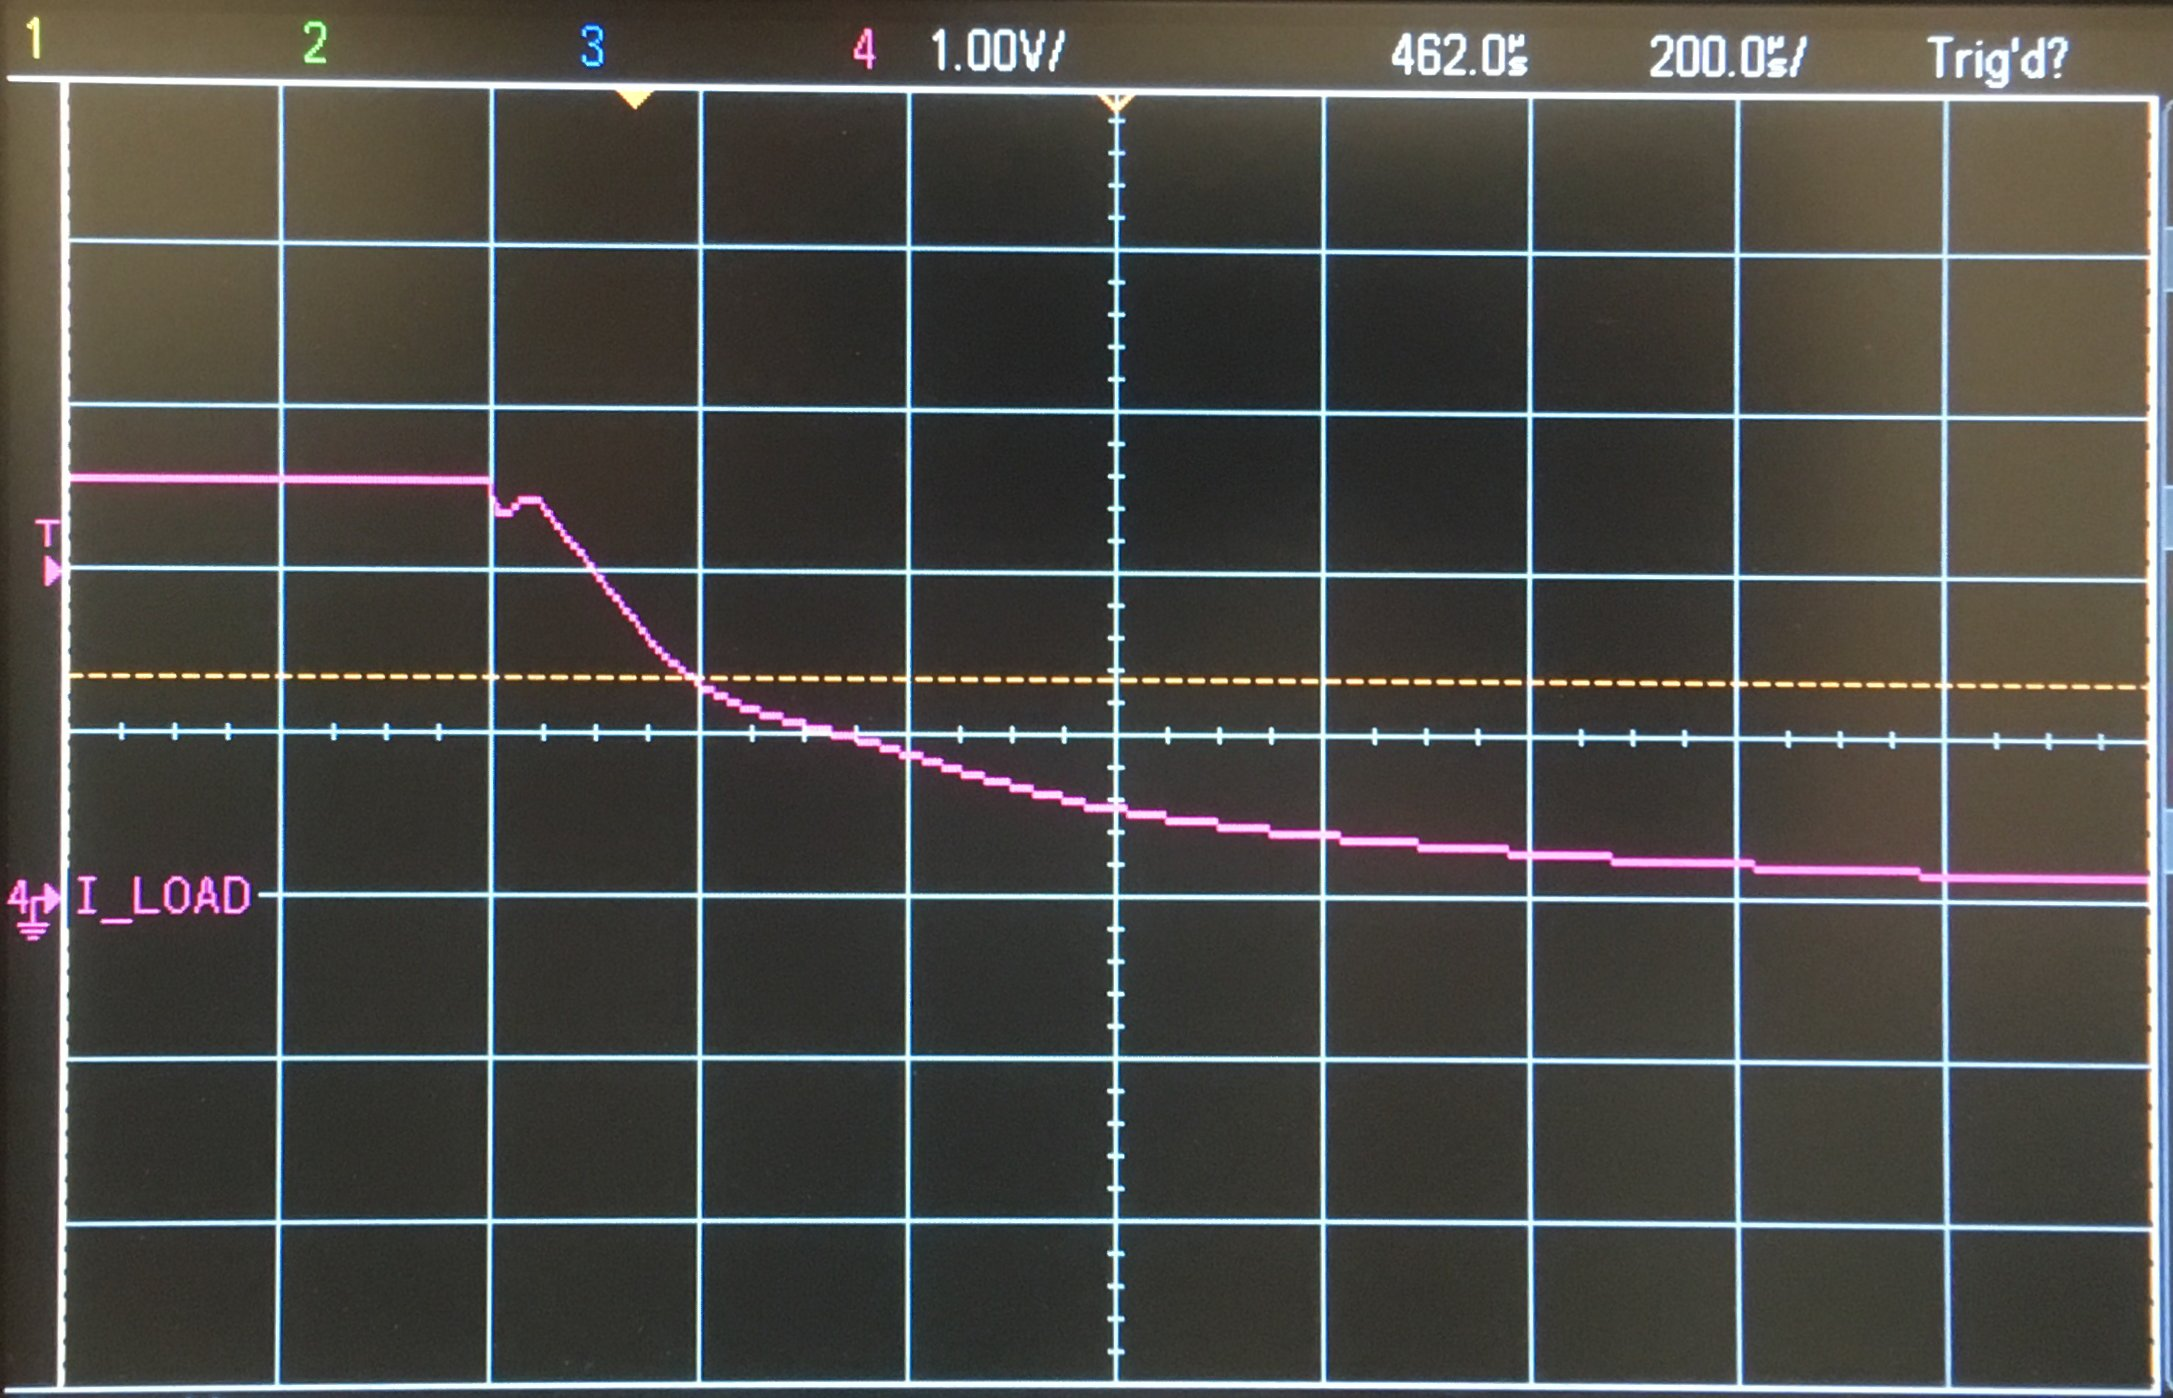
\includegraphics[width=0.8\linewidth]{./res/current_transient/power_off.jpg}
    \caption[Power off transient current]{
        Power off transient current. Measured on 007.
    }
\end{figure}

\begin{figure}[ht]
    \centering
    \begin{subfigure}{0.8\linewidth}
    \begin{tikzpicture}[boximg]
        \node [anchor=south west] (main) {
            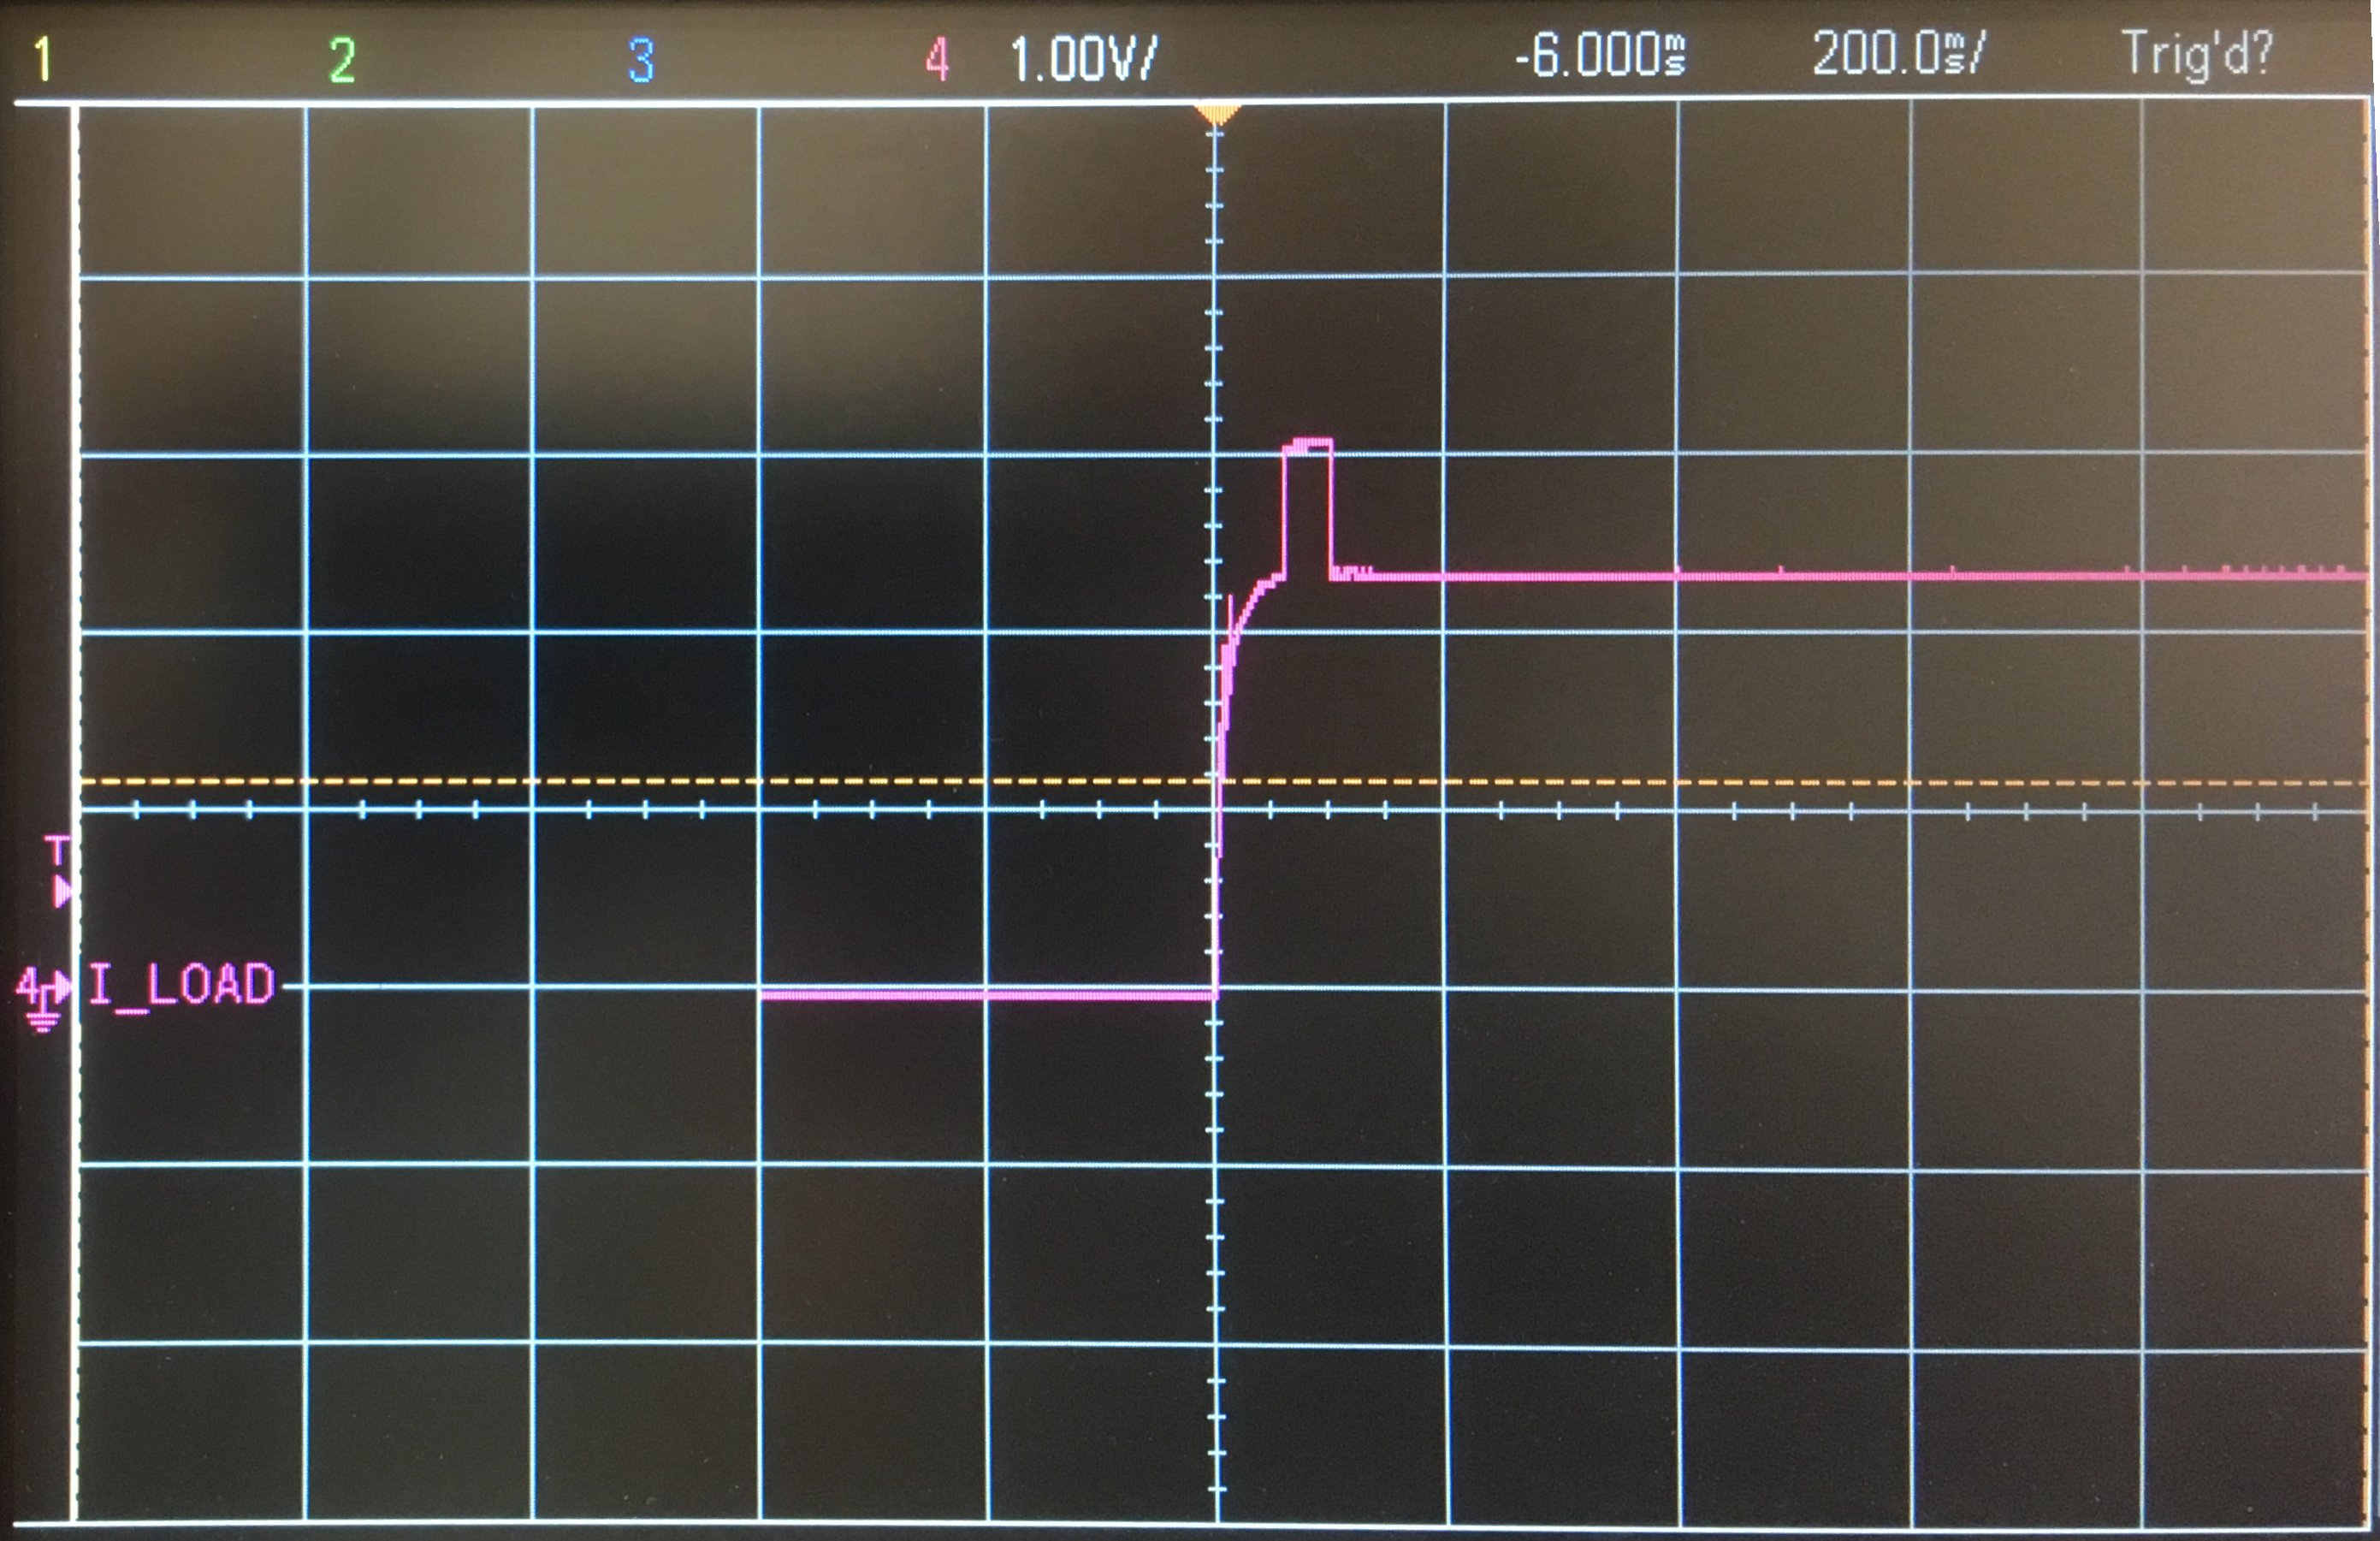
\includegraphics[width=\linewidth]
                {./res/current_transient/power_on.jpg}
        };
        \begin{scope}[x=(main.south east),y=(main.north west)]
            \node [draw,red,minimum height=5em, minimum width=2em] (zoombox1)
                at (0.5,0.5) {};
        \end{scope}
    \end{tikzpicture}
    \caption{}
    \end{subfigure}
    %
    \\[0.5\baselineskip]
    %
    \begin{subfigure}{0.5\linewidth}
    \begin{tikzpicture}[boximg,red]
        \node (zoom1) {
            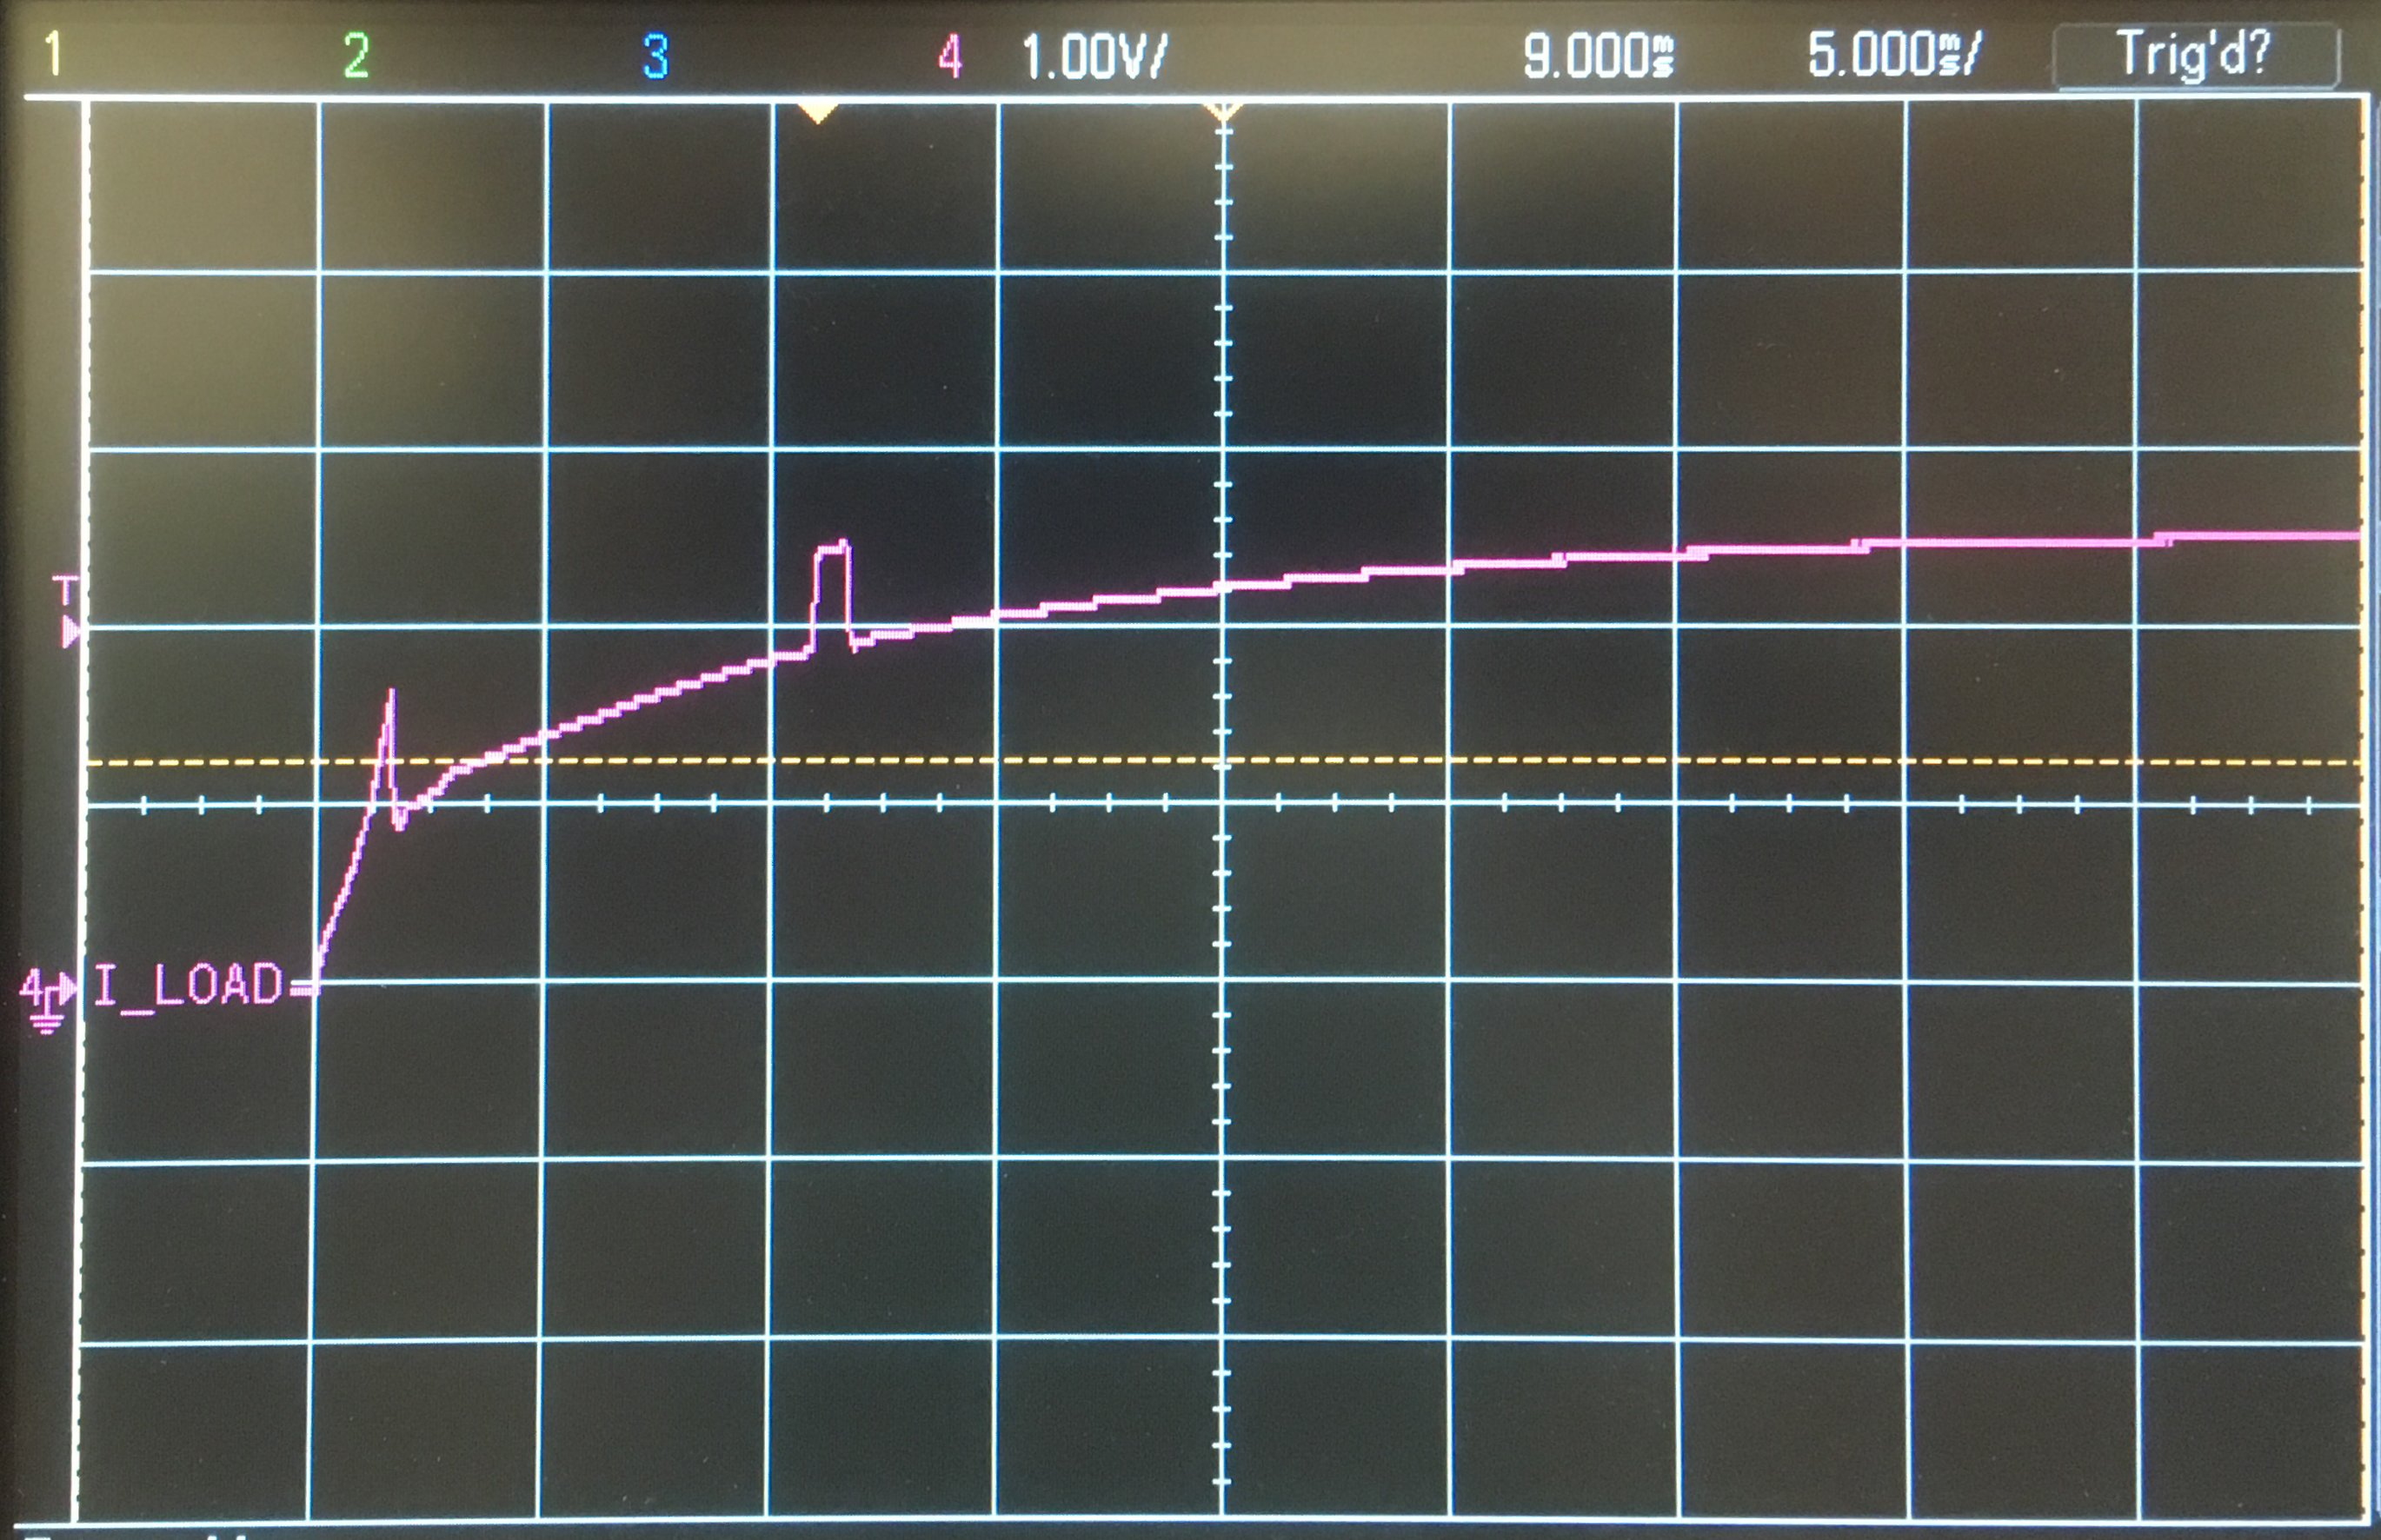
\includegraphics[width=\linewidth]
                {./res/current_transient/power_on-zoom.jpg}
        };
        \draw (zoom1.south west) rectangle (zoom1.north east);
    \end{tikzpicture}
    \caption{}
    \end{subfigure}
    %\begin{tikzpicture}[overlay,boximg]
        %\draw (zoom1) -- (zoombox1);
    %\end{tikzpicture}
    \caption[Power on transient current]{
        Power on transient current. Measured on 007.
    }
\end{figure}

\begin{figure}[ht]
    \centering
    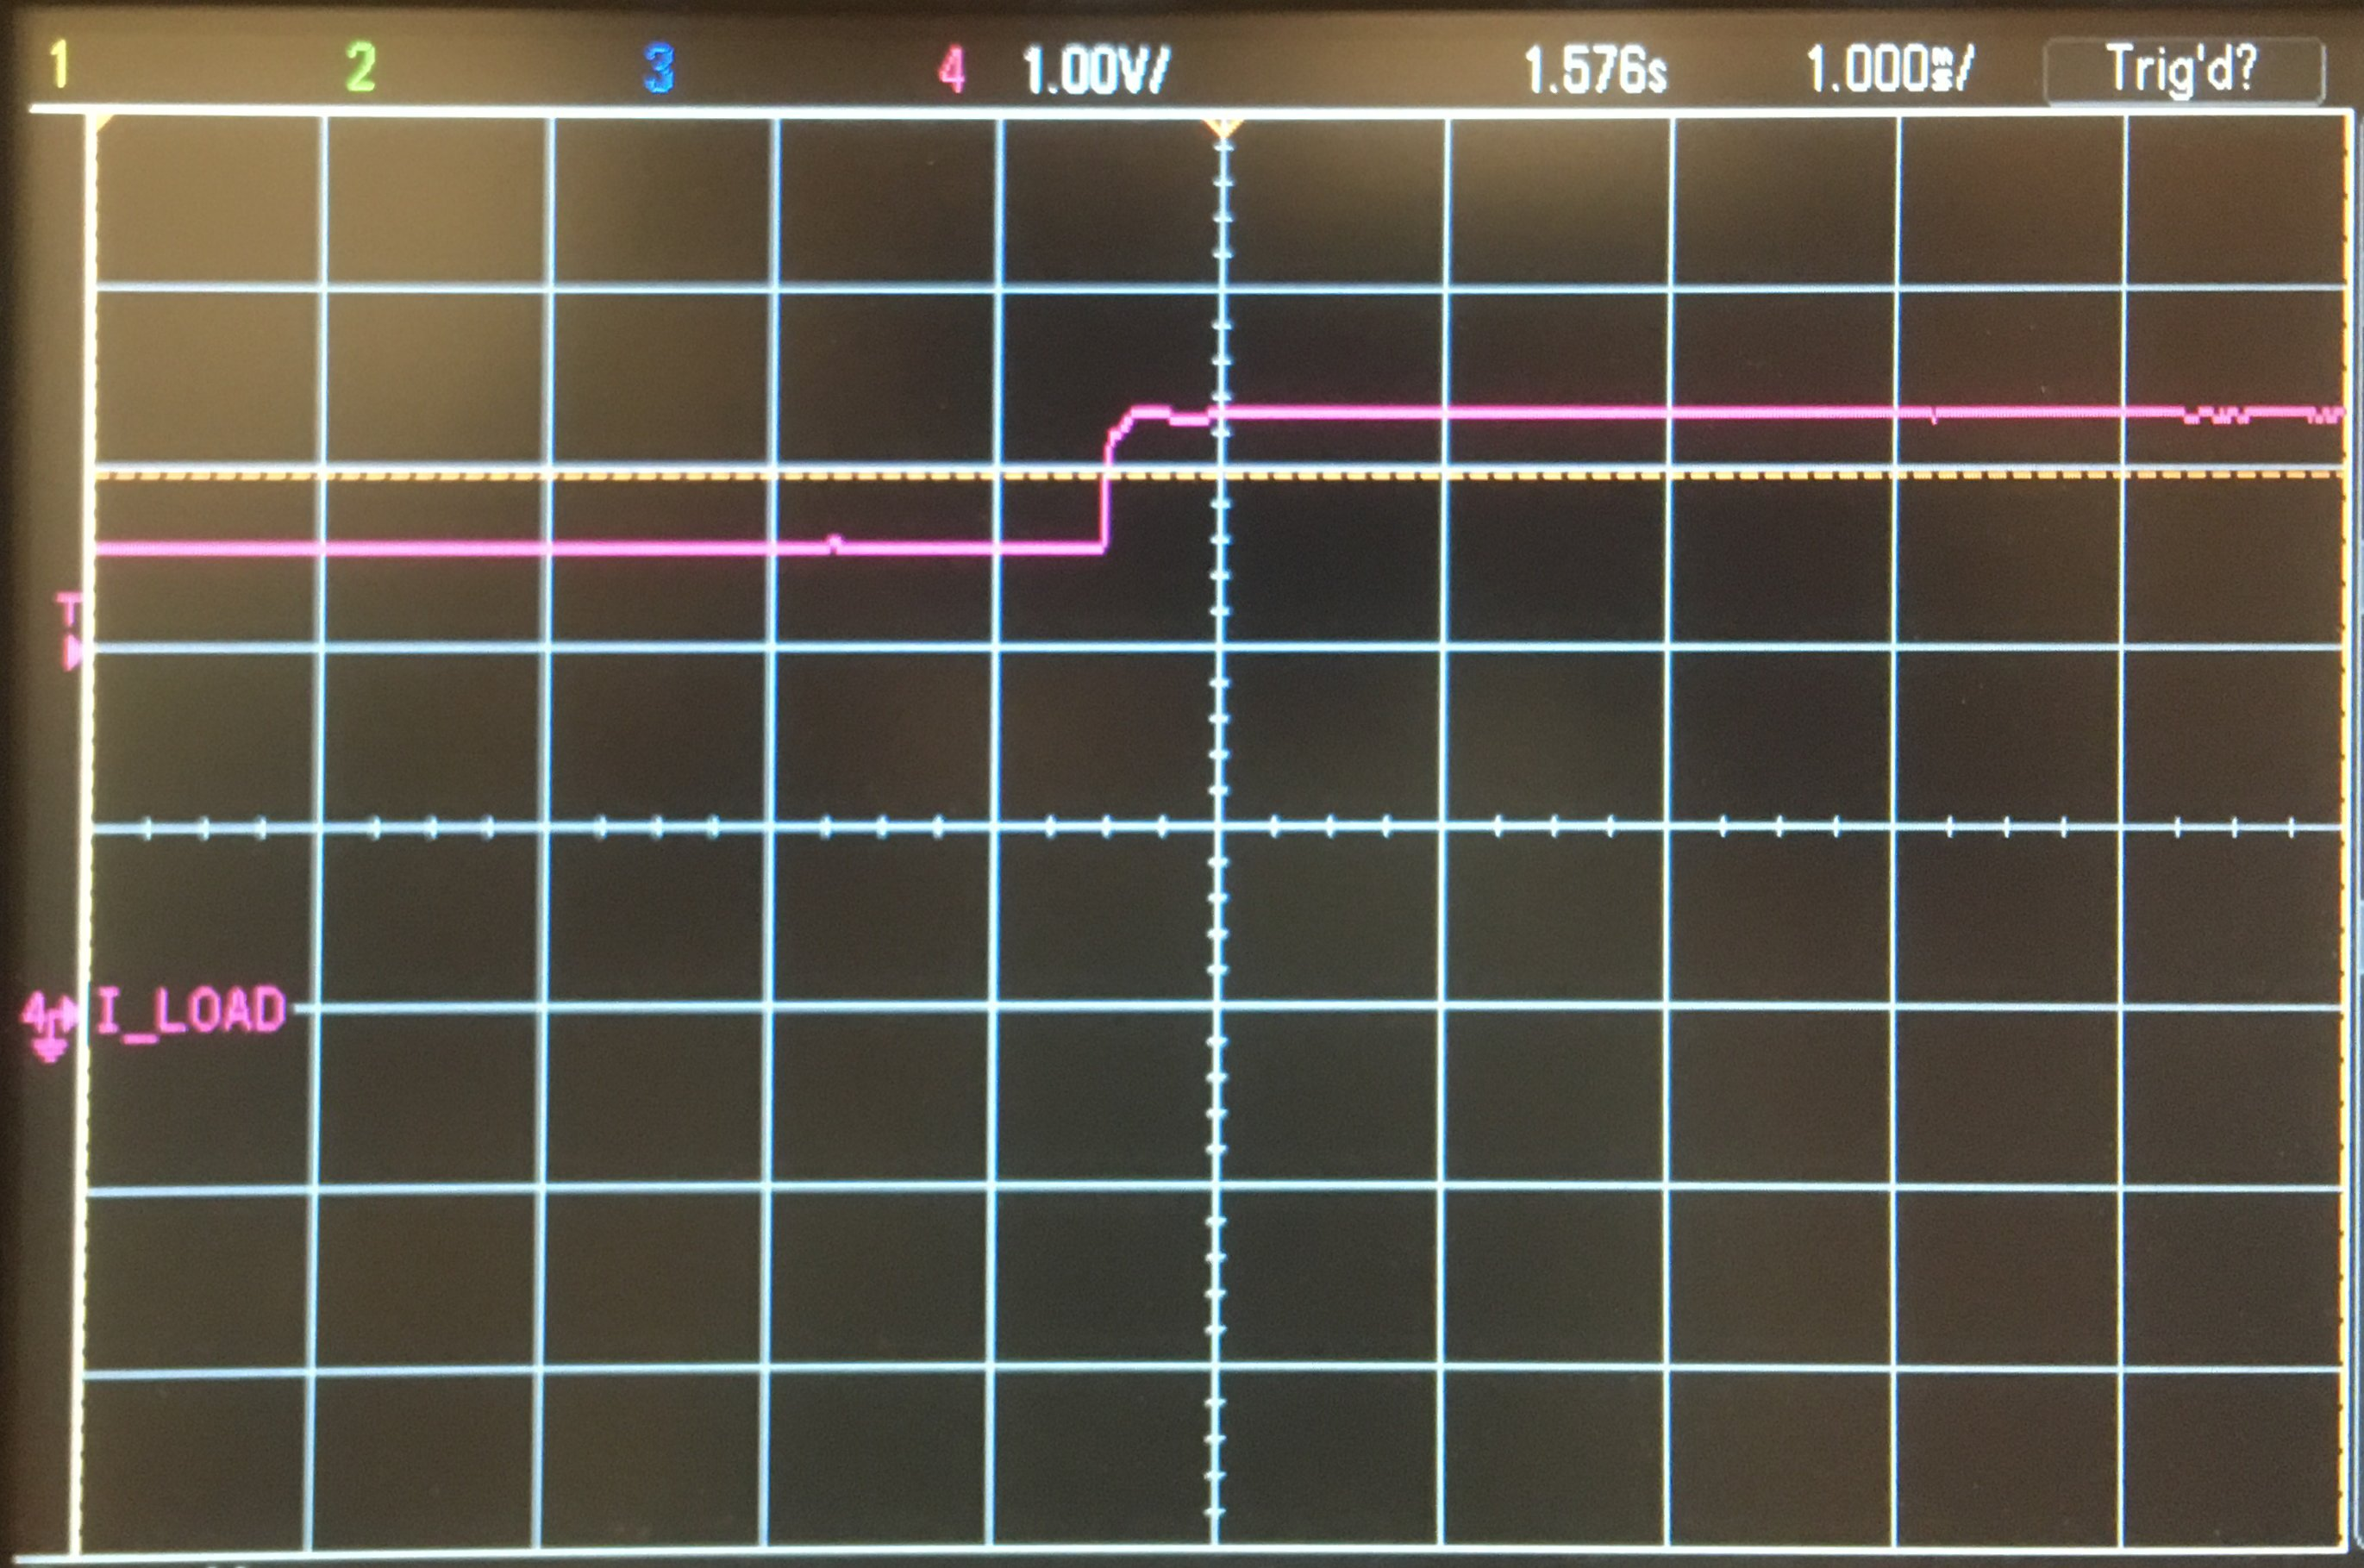
\includegraphics[width=0.8\linewidth]
        {./res/current_transient/program_master.jpg}
    \caption[Program master GBTx transient current]{
        Program master GBTx (via \itwoc) transient current.
        Measured on 007.
    }
\end{figure}

\begin{figure}[ht]
    \centering
    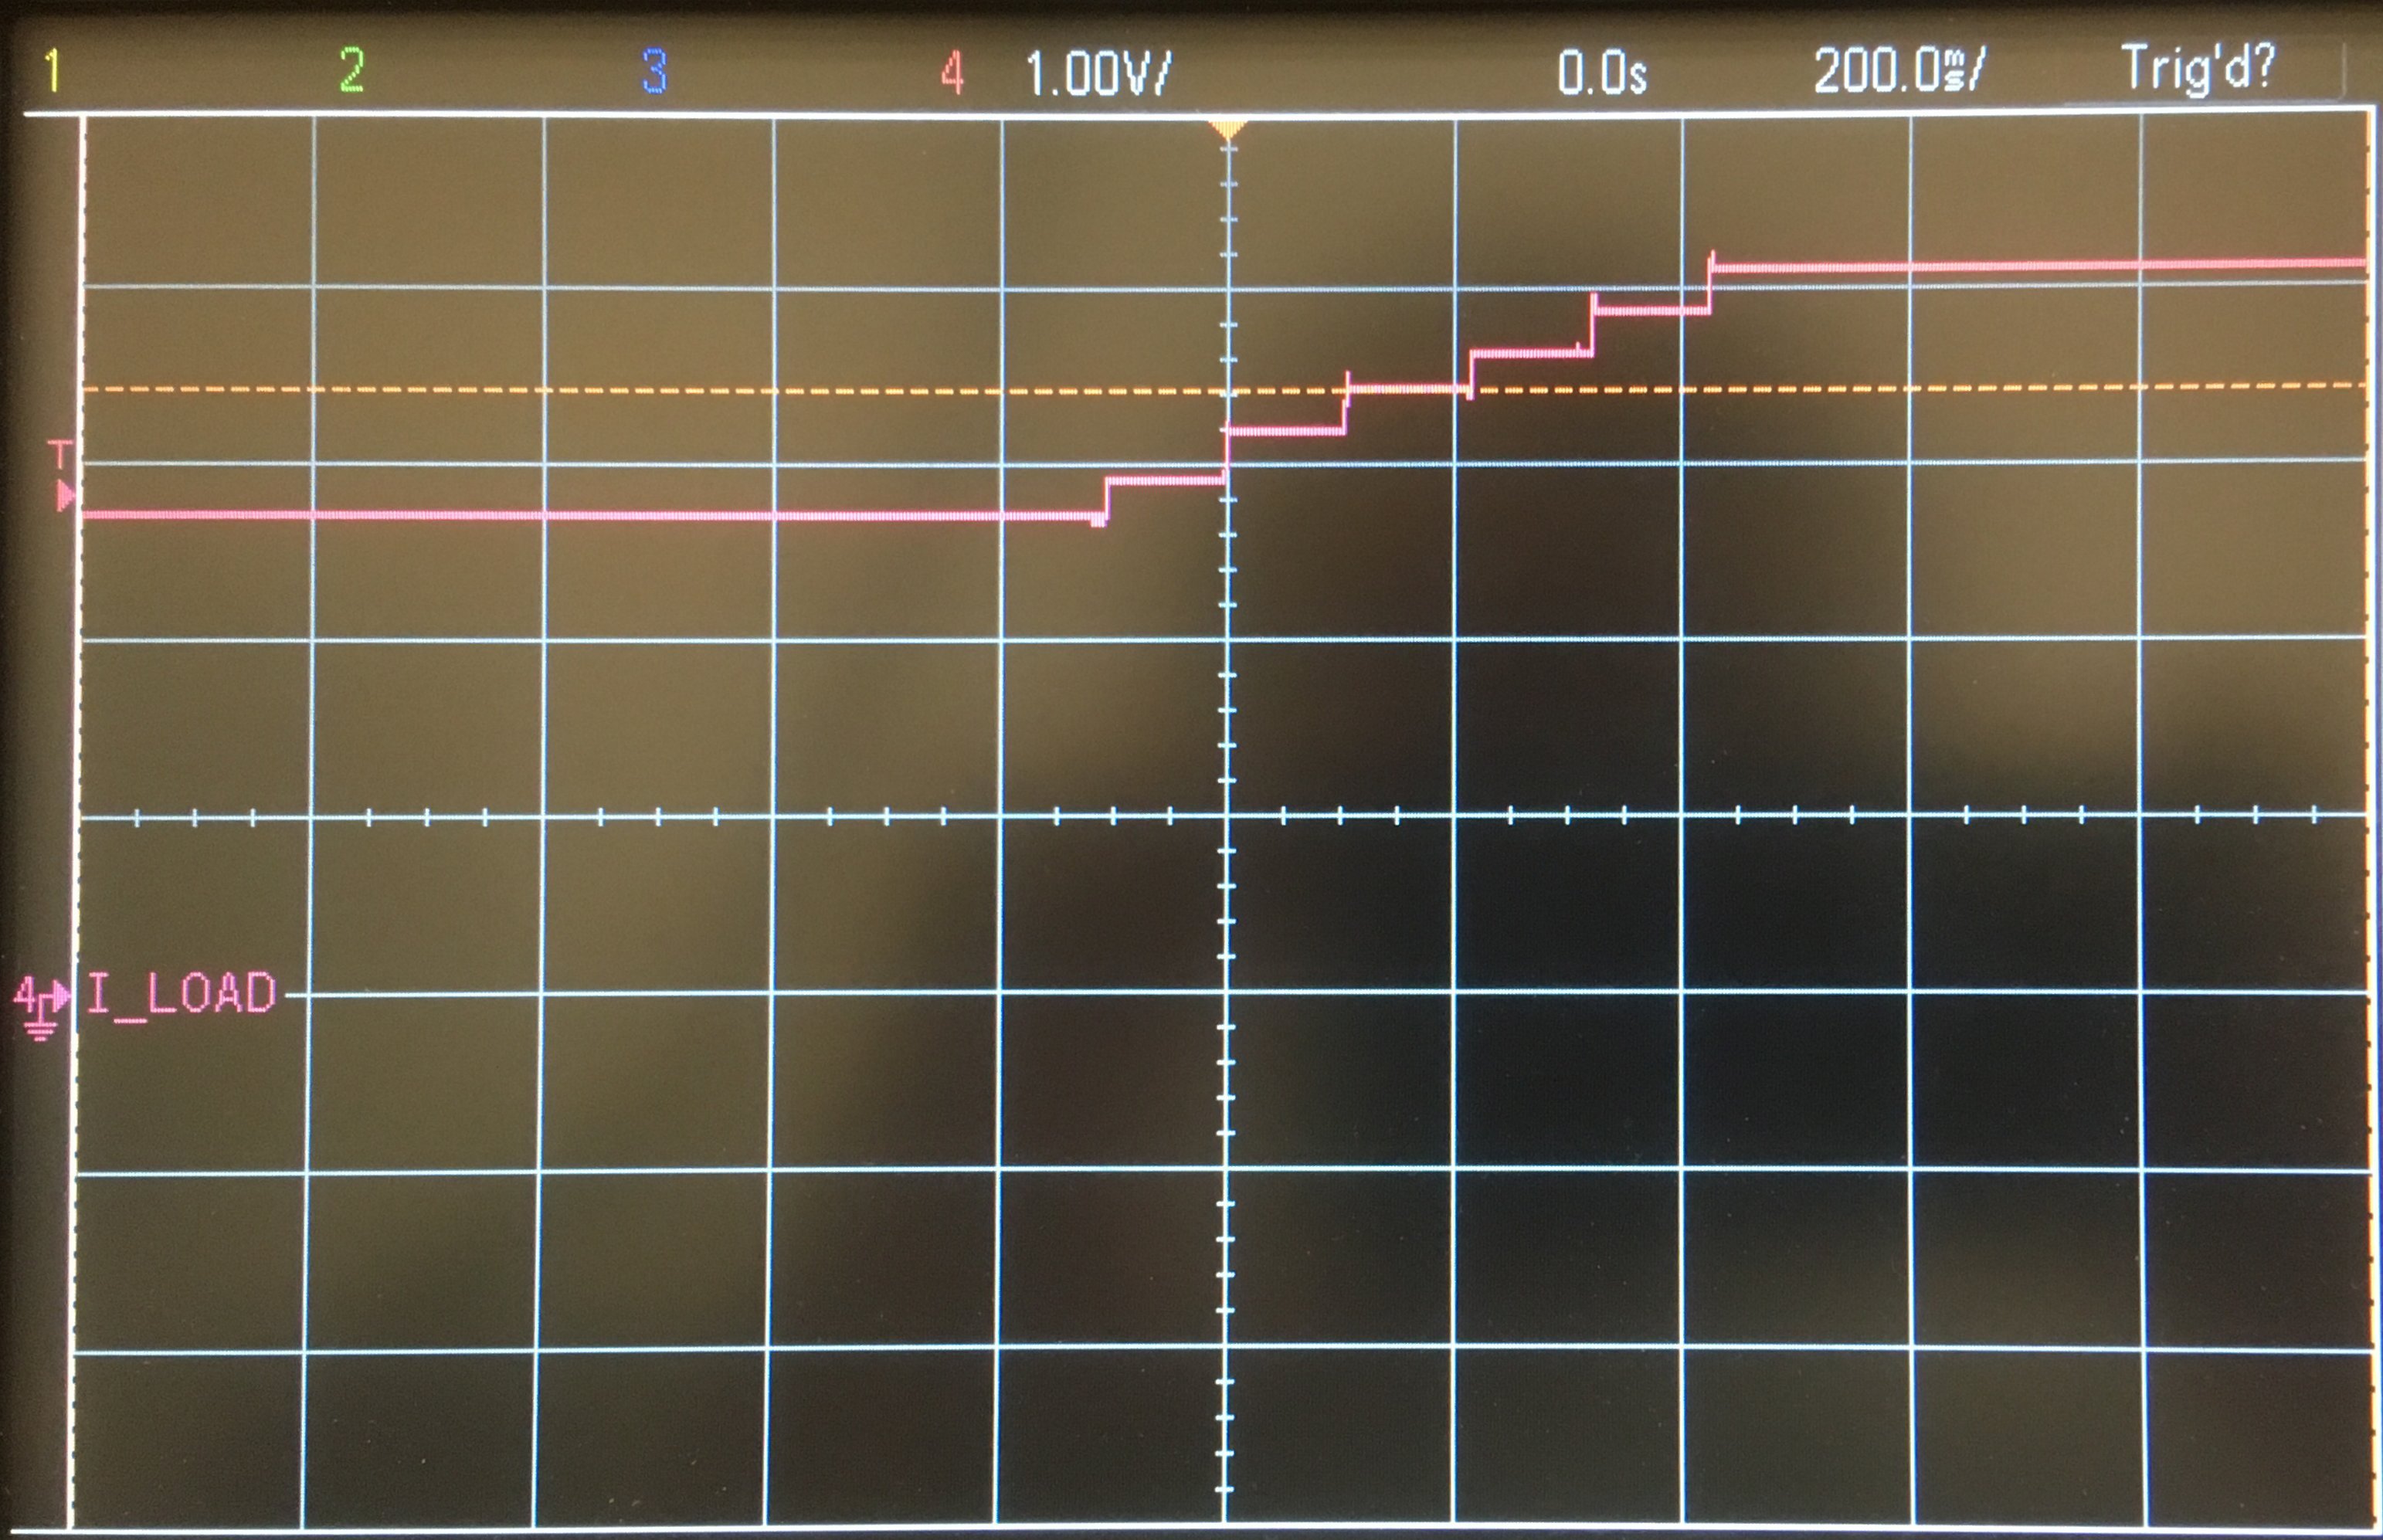
\includegraphics[width=0.8\linewidth]
        {./res/current_transient/program_data.jpg}
    \caption[Program data GBTxs transient current]{
        Program all 6 data GBTxs (via GBT-IC) transient current.
        The programmer on MiniDAQ is written in a way such that these data GBTxs
        are programmed one by one.
        Measured on 007.
    }
\end{figure}

\begin{figure}[ht]
    \centering
    \begin{subfigure}{0.8\linewidth}
    \begin{tikzpicture}[boximg]
        \node [anchor=south west] (main) {
            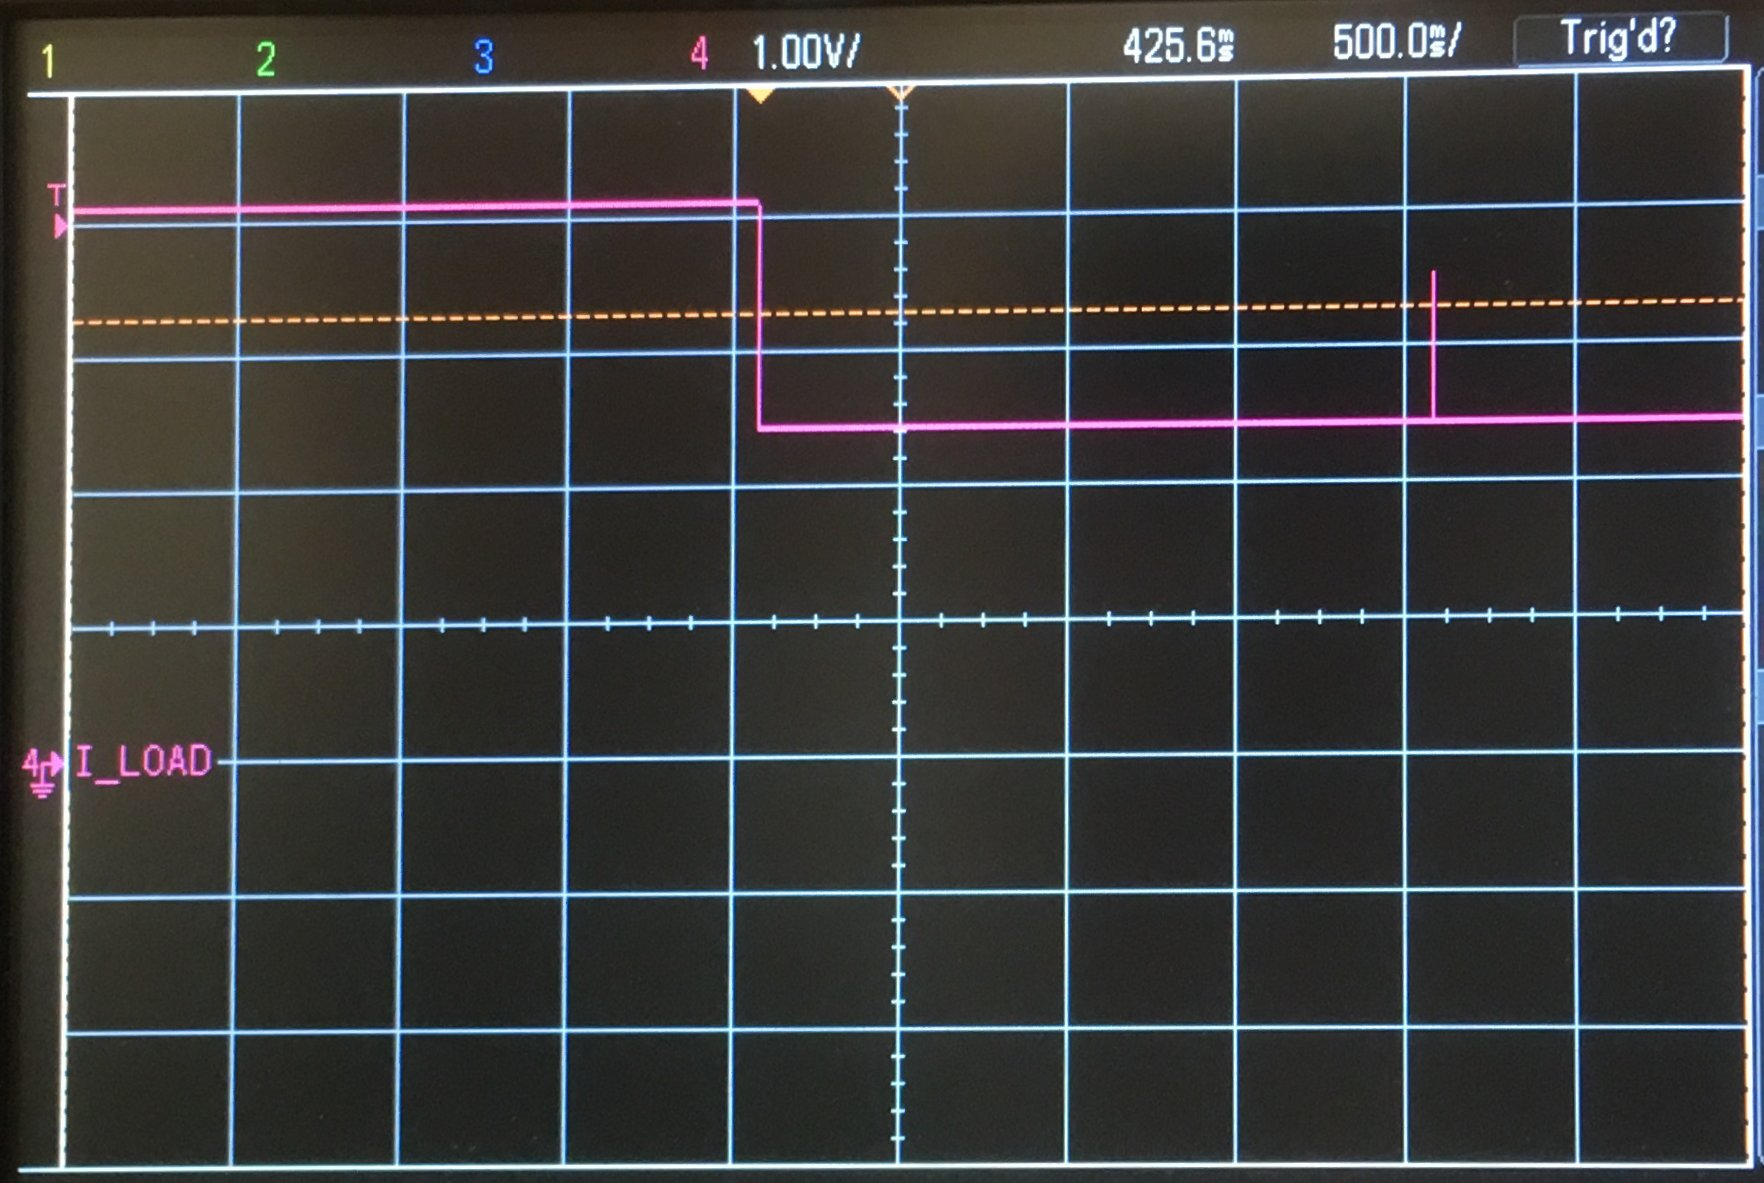
\includegraphics[width=\linewidth]
            {./res/current_transient/loss_of_lock.jpg}
        };
        \begin{scope}[x=(main.south east),y=(main.north west)]
            \node [draw,red,minimum height=4.5em, minimum width=1.5em]
                (zoombox1) at (0.42,0.72) {};
            \node [draw,green,minimum height=3.5em, minimum width=1.5em]
                (zoombox2) at (0.81,0.7) {};
        \end{scope}
    \end{tikzpicture}
    \caption{}
    \end{subfigure}
    %
    \\[0.5\baselineskip]
    %
    \begin{subfigure}{0.38\linewidth}
    \begin{tikzpicture}[boximg,red]
        \node (zoom1) {
            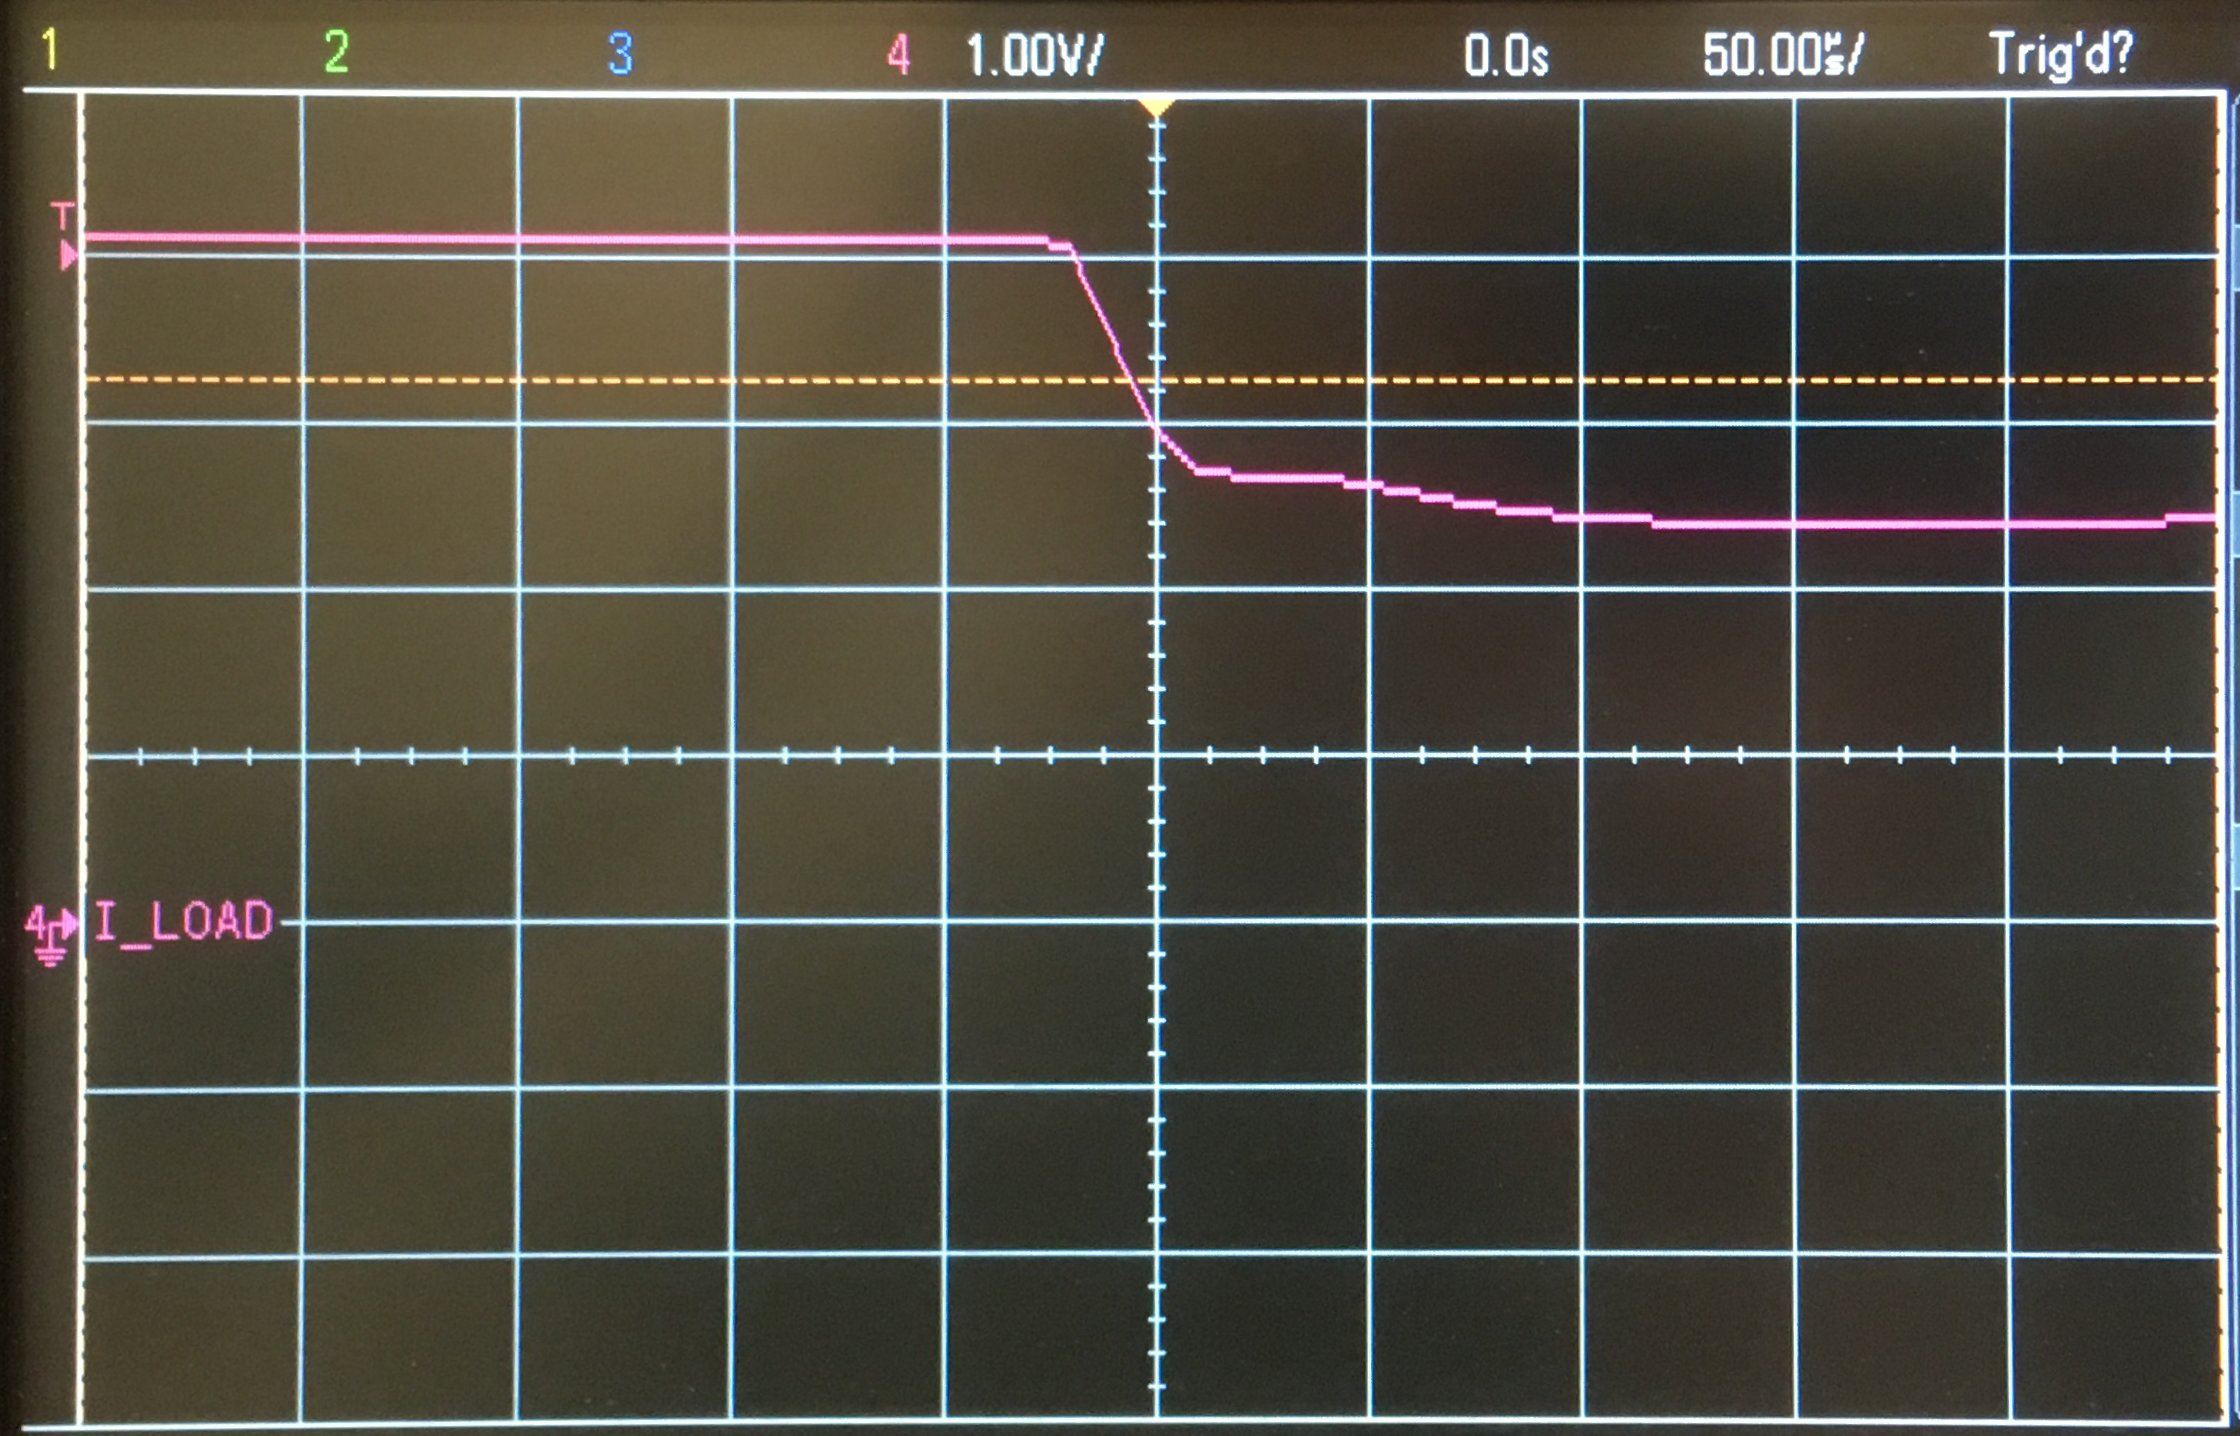
\includegraphics[width=\linewidth]
                {./res/current_transient/loss_of_lock-zoom1.jpg}
        };
        \draw (zoom1.south west) rectangle (zoom1.north east);
    \end{tikzpicture}
    \caption{}
    \end{subfigure}
    %
    \hspace{0.02\linewidth}
    %
    \begin{subfigure}{0.38\linewidth}
    \begin{tikzpicture}[boximg,green]
        \node  (zoom2) {
            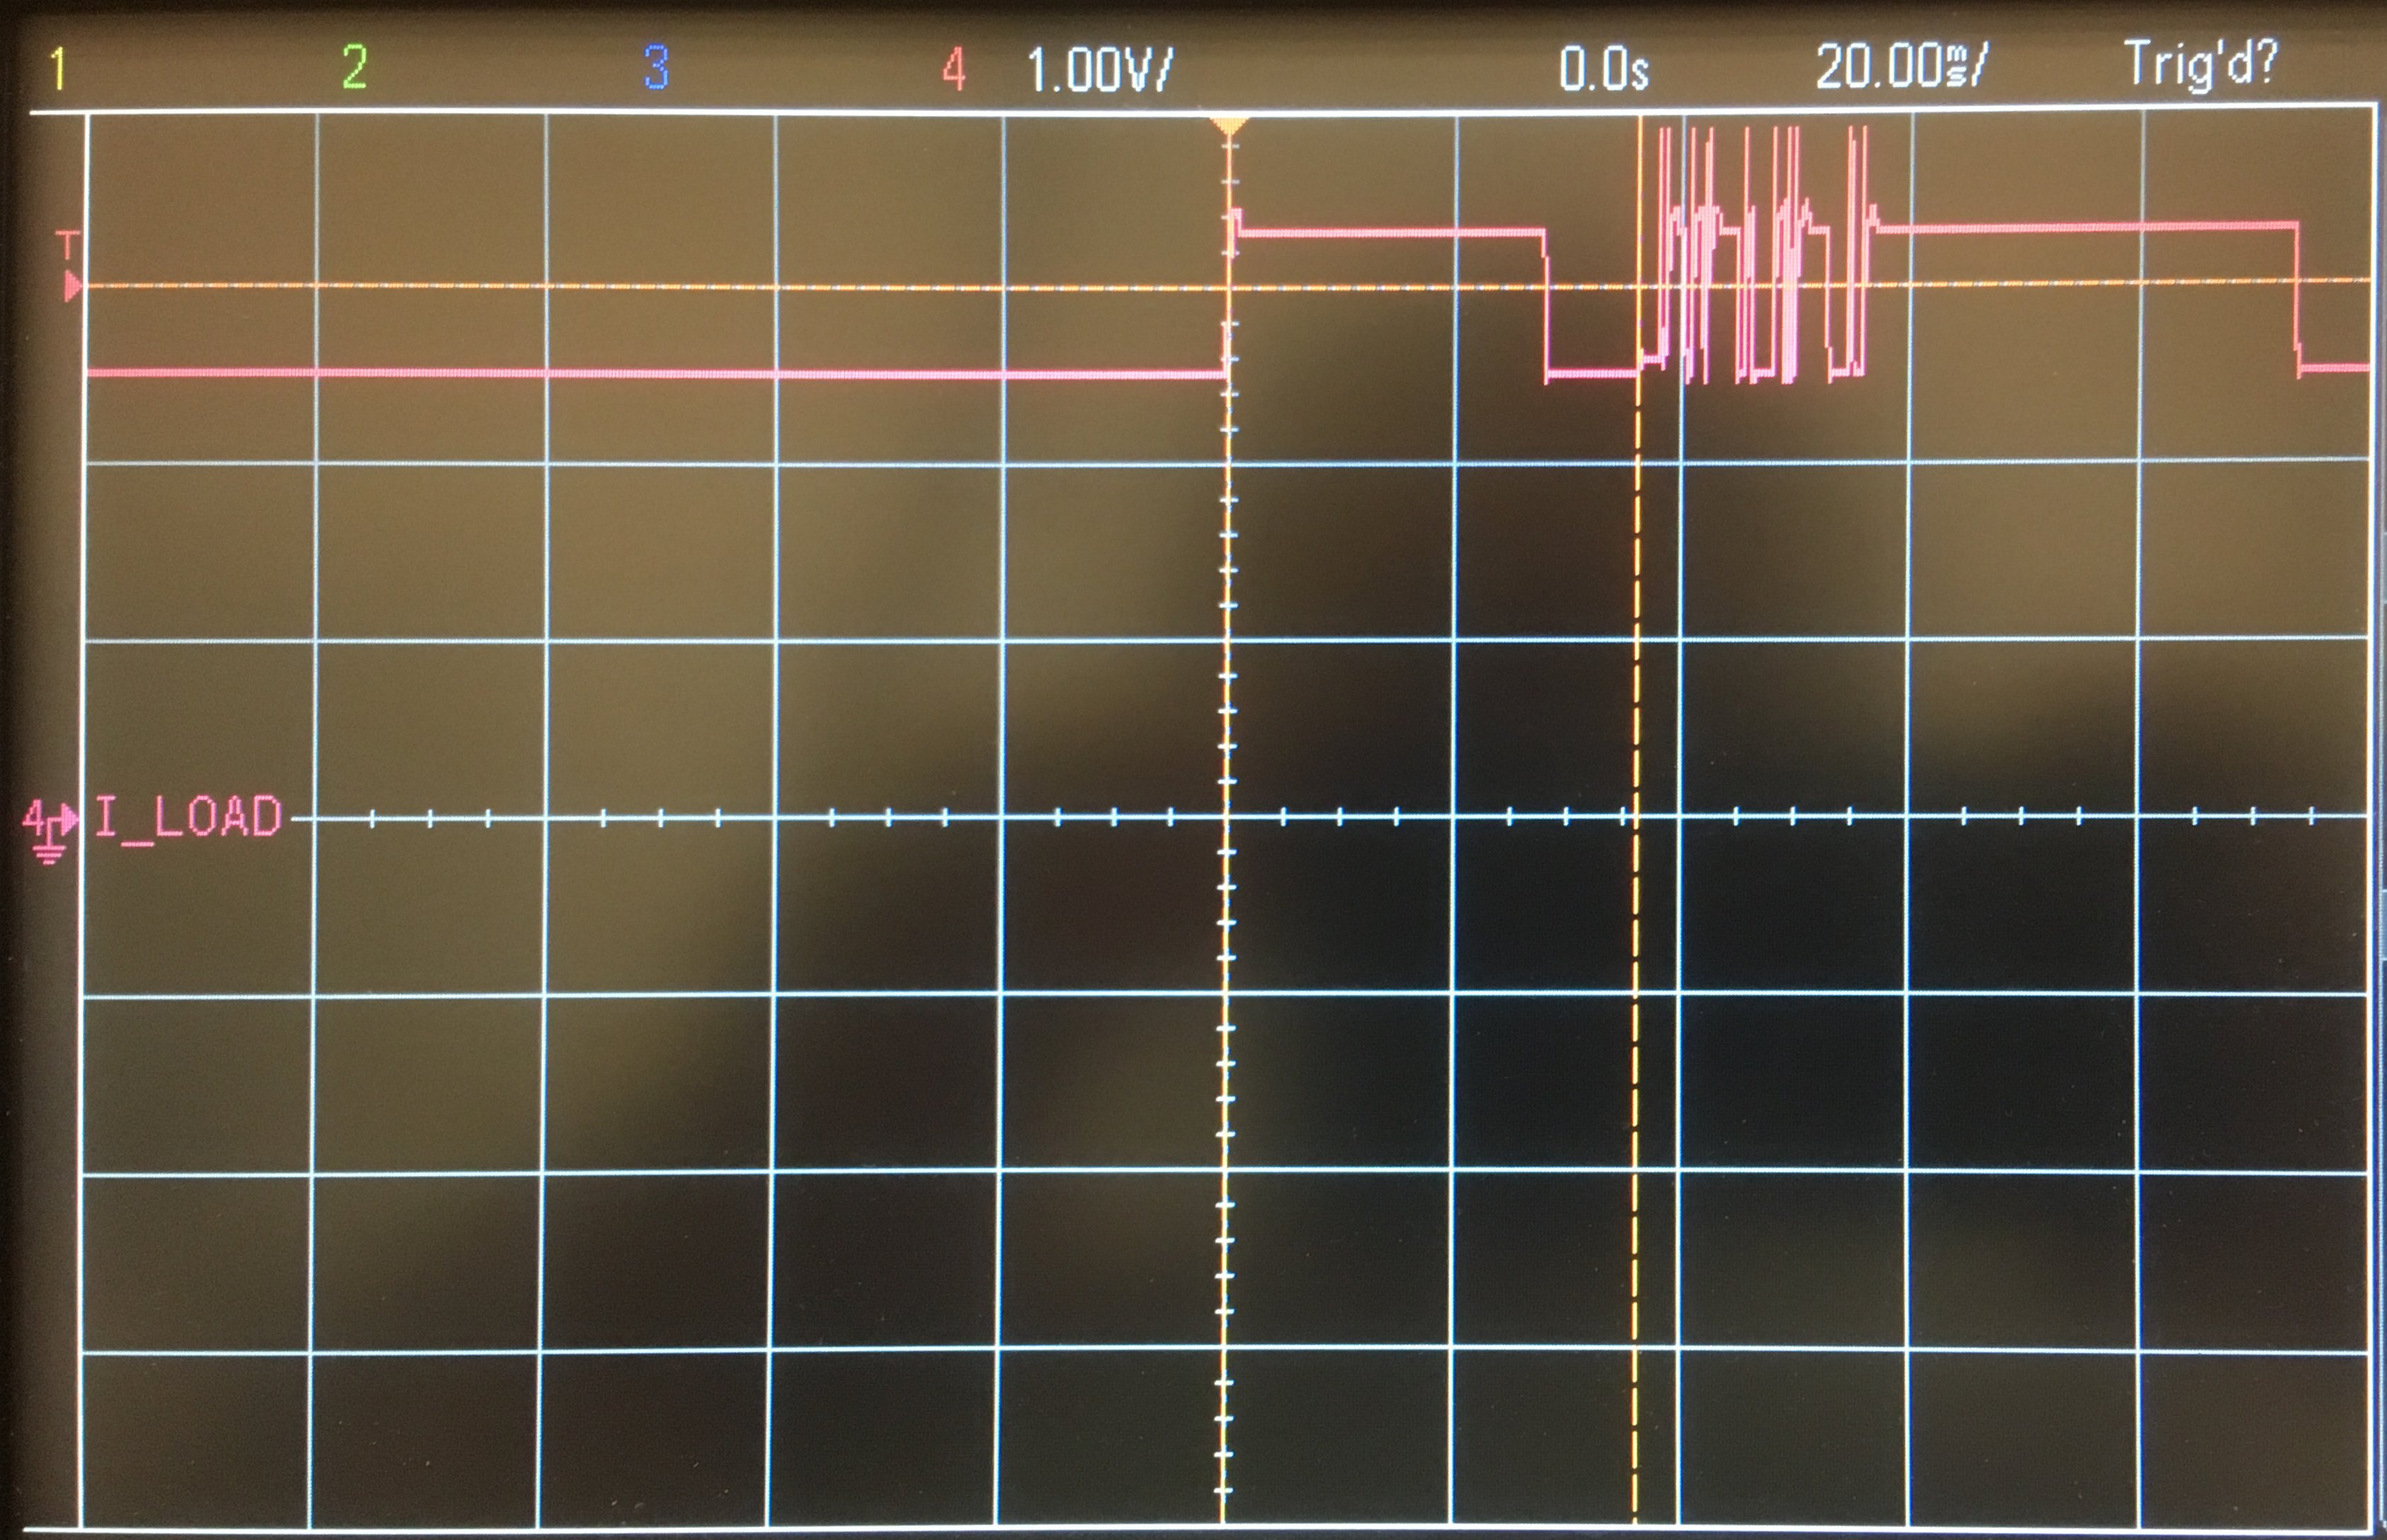
\includegraphics[width=\linewidth]
                {./res/current_transient/loss_of_lock-zoom2.jpg}
        };
        \draw (zoom2.south west) rectangle (zoom2.north east);
    \end{tikzpicture}
    \caption{}
    \end{subfigure}
    %
    \caption[Loss of lock transient current]{
        Loss of lock transient current. Measured on 007.
    }
\end{figure}

\begin{figure}[ht]
    \centering
    \begin{subfigure}{0.8\linewidth}
    \begin{tikzpicture}[boximg]
        \node [anchor=south west] (main) {
            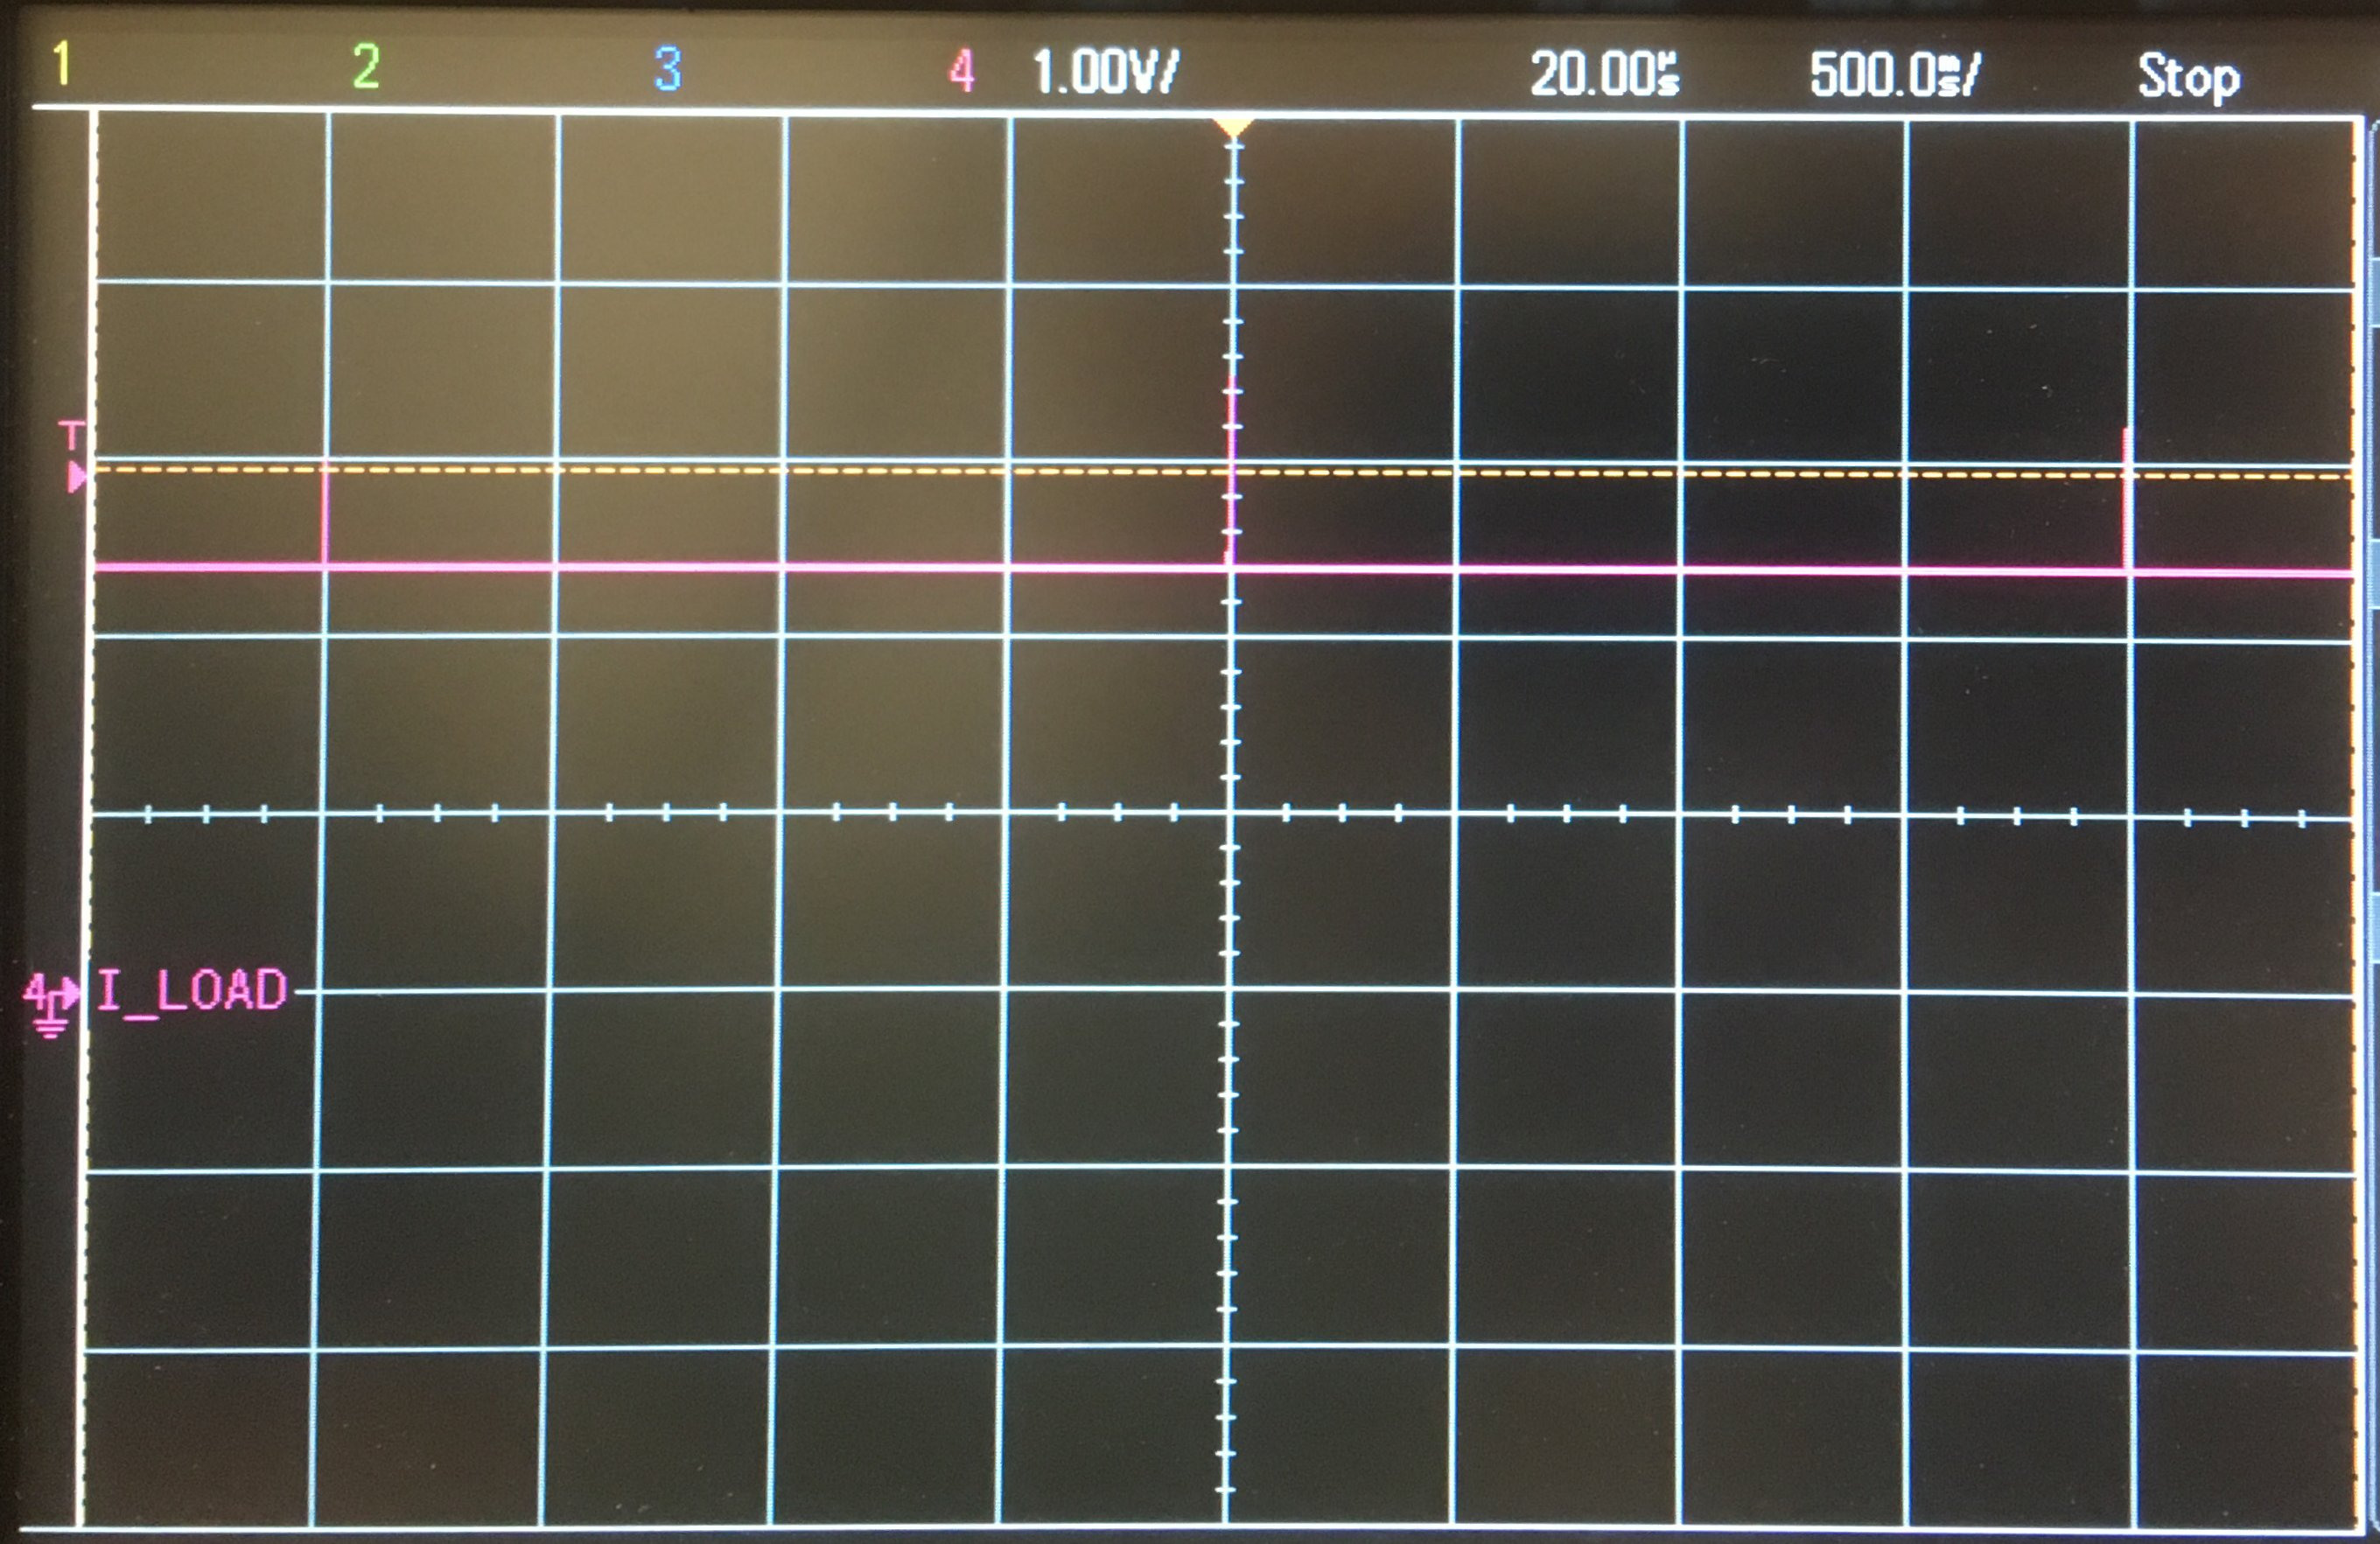
\includegraphics[width=\linewidth]
            {./res/current_transient/during_loss_of_lock.jpg}
        };
        \begin{scope}[x=(main.south east),y=(main.north west)]
            \node [draw,red,minimum height=4.5em, minimum width=1.5em]
                (zoombox1) at (0.52,0.7) {};
        \end{scope}
    \end{tikzpicture}
    \caption{}
    \end{subfigure}
    %
    \\[0.5\baselineskip]
    %
    \begin{subfigure}{0.42\linewidth}
    \begin{tikzpicture}[boximg,red]
        \node [anchor=south west] (zoom1) {
            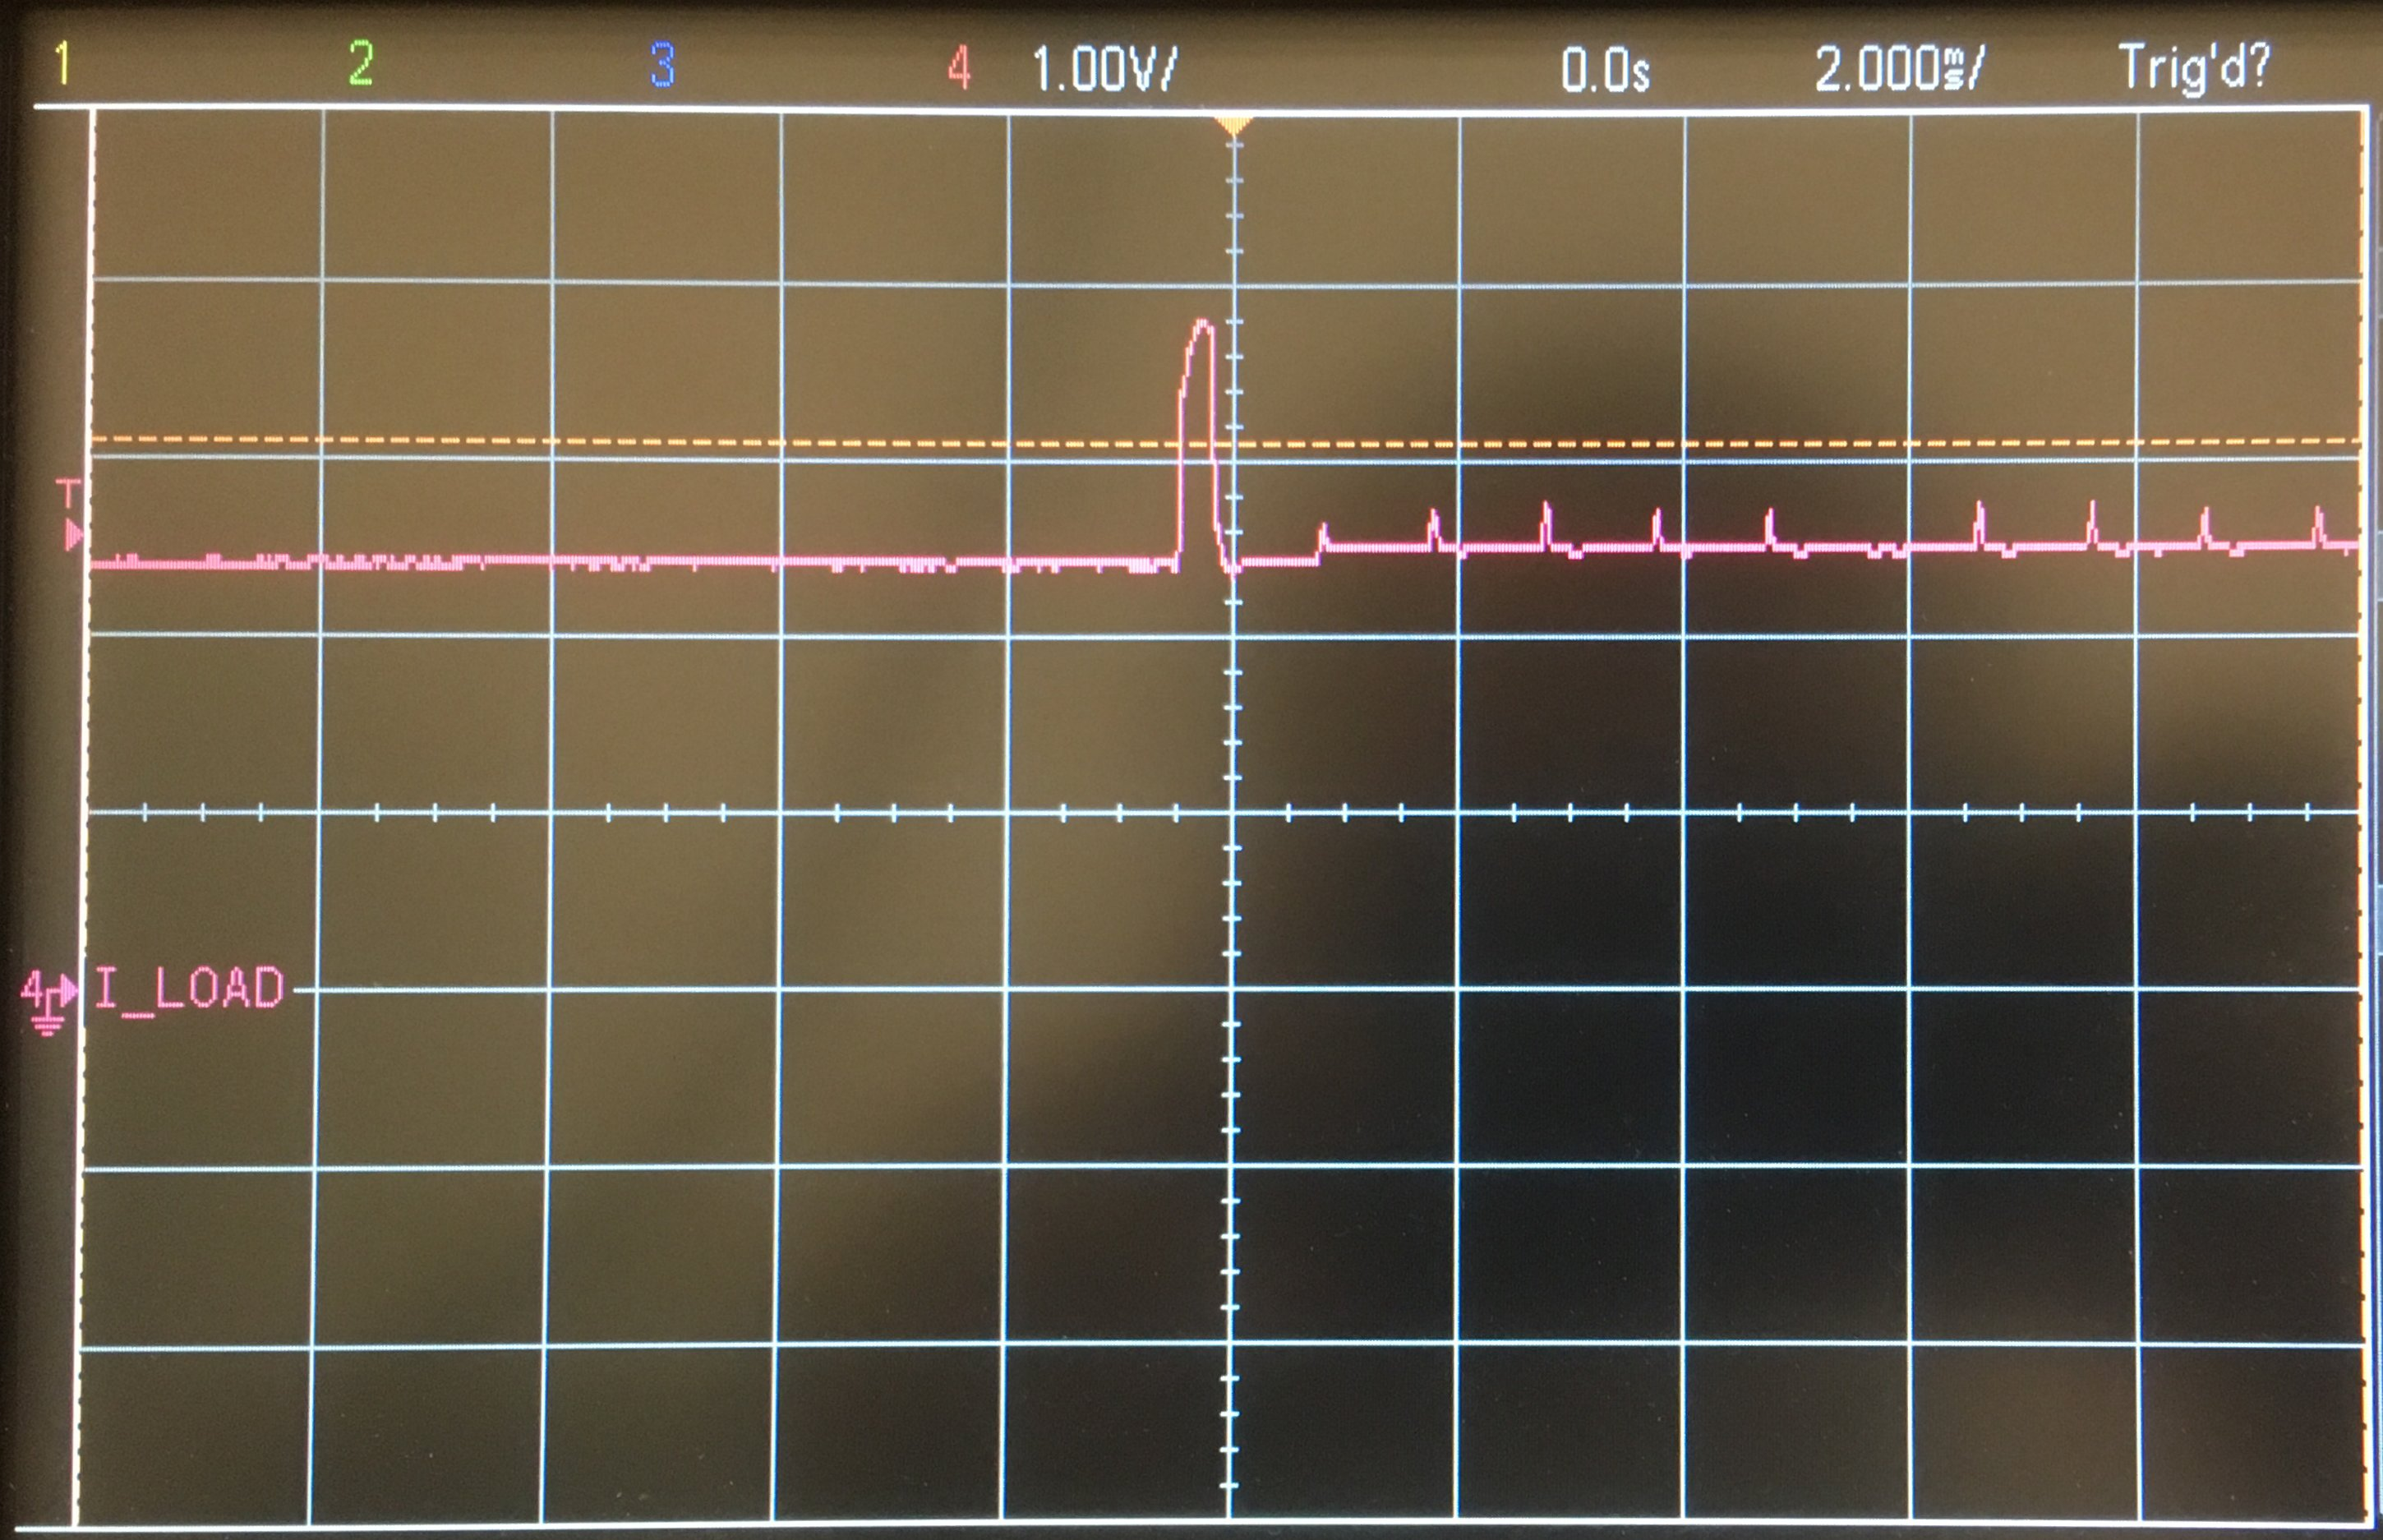
\includegraphics[width=\linewidth]
                {./res/current_transient/during_loss_of_lock-zoom.jpg}
        };
        \draw (zoom1.south west) rectangle (zoom1.north east);
        \begin{scope}[x=(zoom1.south east),y=(zoom1.north west)]
            \node [draw,green,minimum height=2em, minimum width=1em]
                (zoombox2) at (0.5,0.7) {};
        \end{scope}
    \end{tikzpicture}
    \caption{}
    \end{subfigure}
    %
    \hspace{0.04\linewidth}
    %
    \begin{subfigure}{0.32\linewidth}
    \begin{tikzpicture}[boximg,green]
        \node  (zoom2) {
            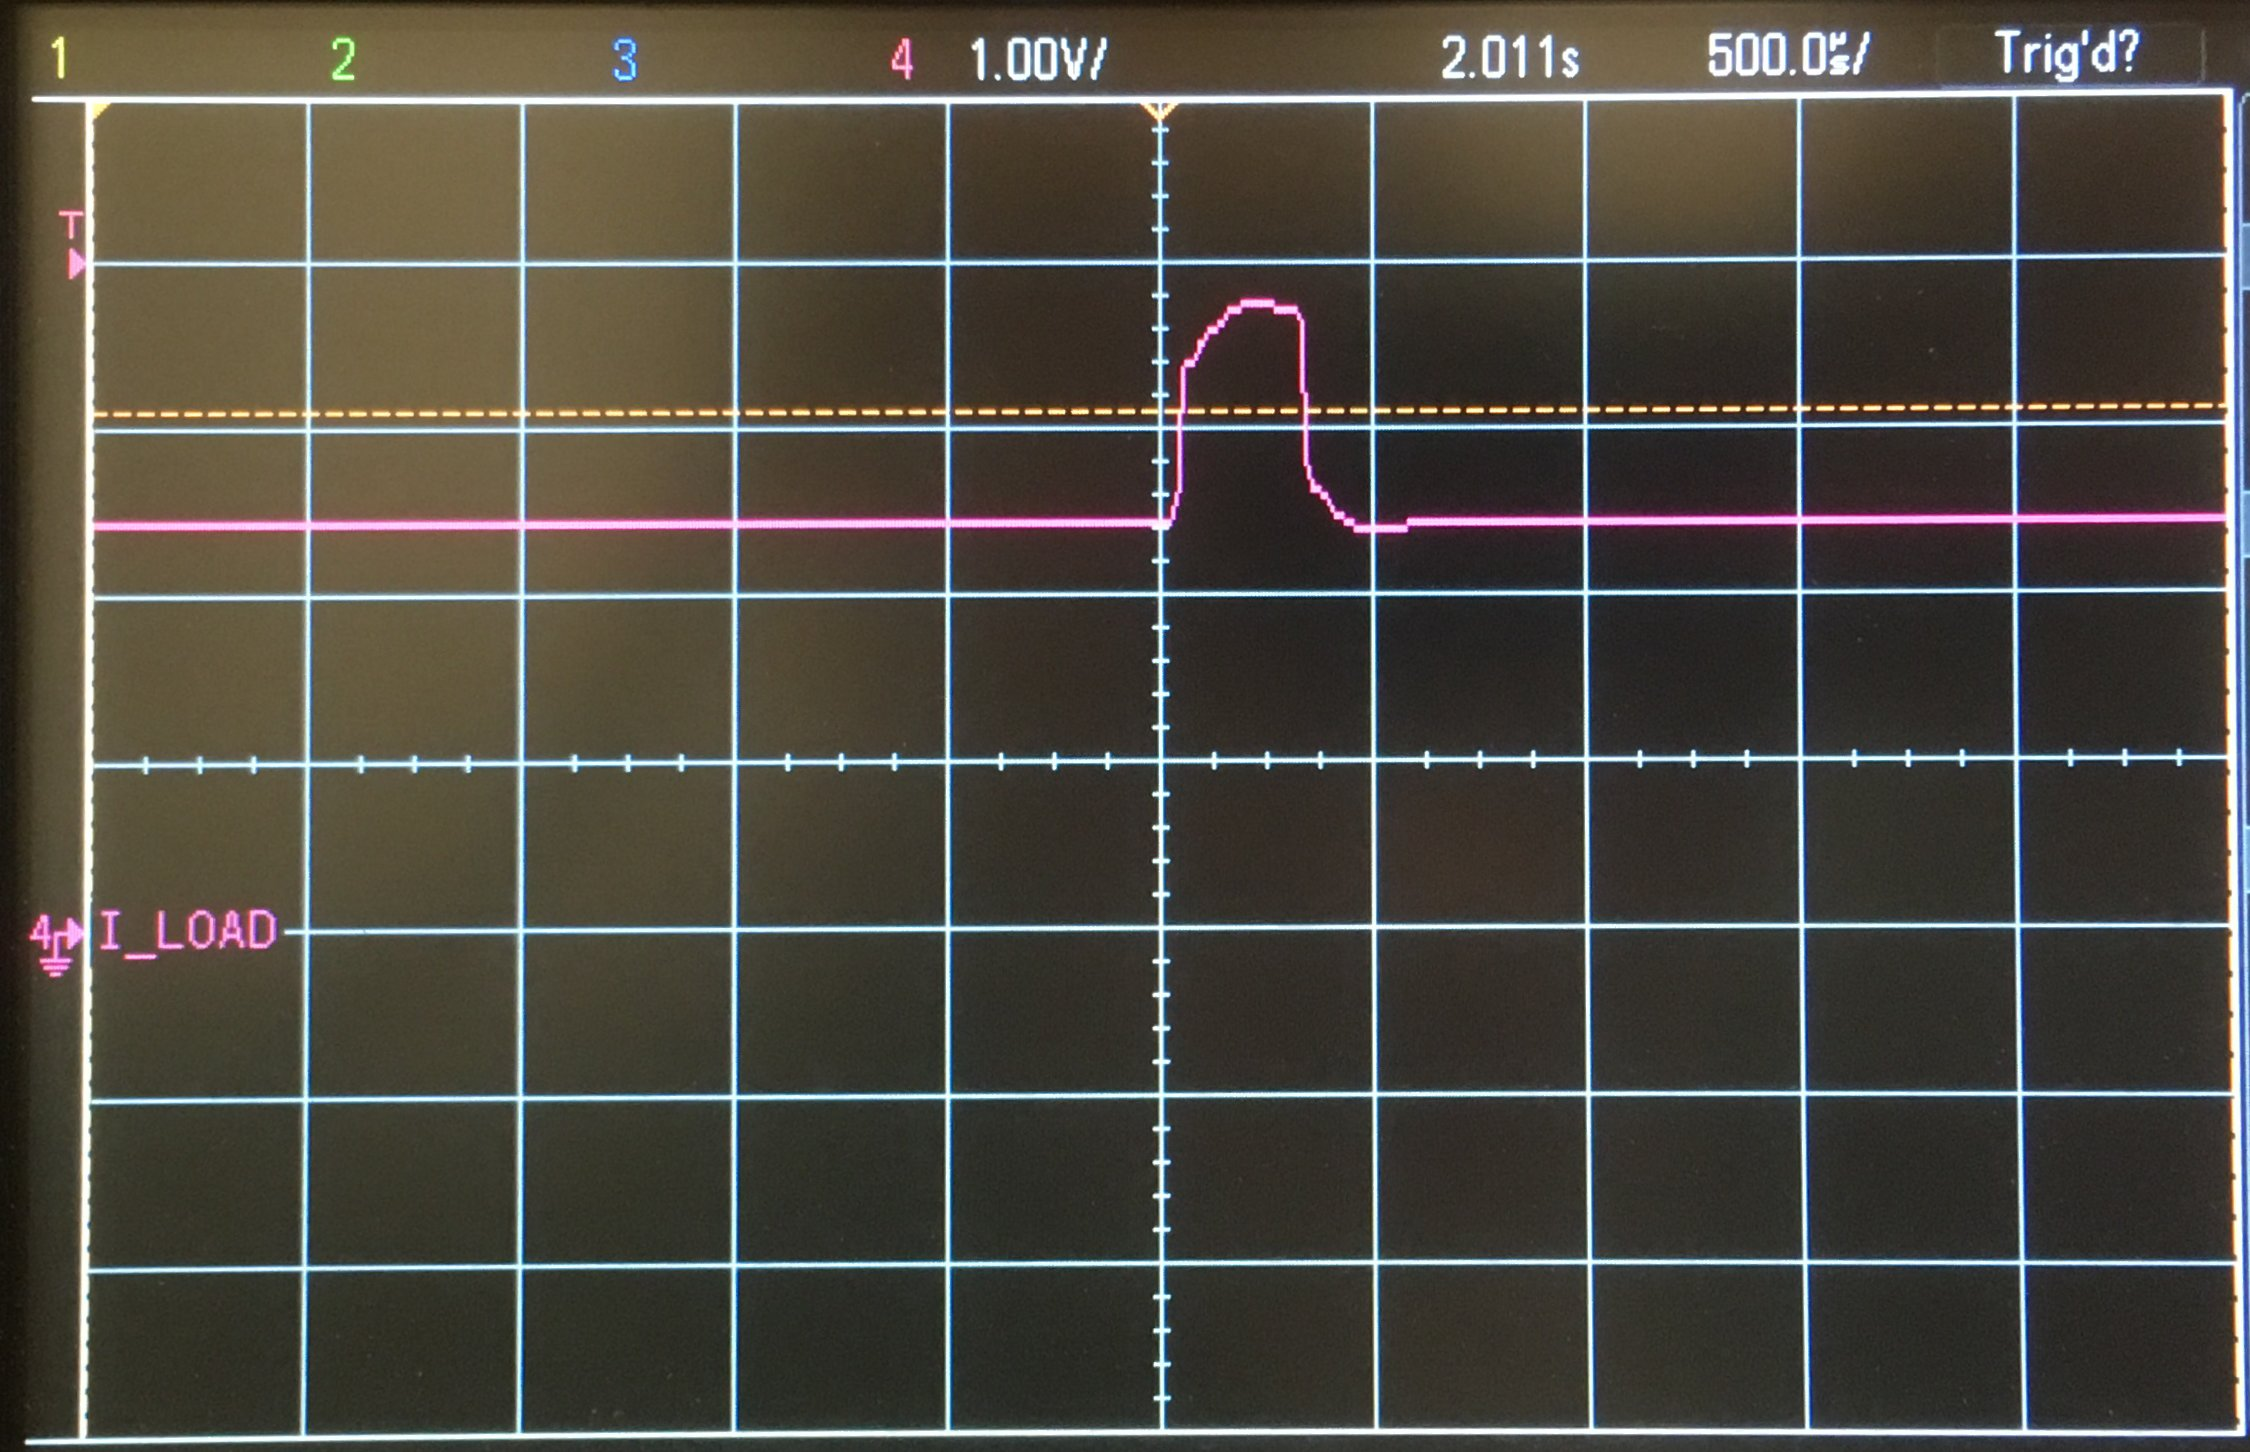
\includegraphics[width=\linewidth]
                {./res/current_transient/during_loss_of_lock-zoom-zoom.jpg}
        };
        \draw (zoom2.south west) rectangle (zoom2.north east);
    \end{tikzpicture}
    \caption{}
    \end{subfigure}
    %
    \caption[During loss of lock transient current]{
        During loss of lock transient current.
        DCB 007 in this stage is cleaner than DCB 008.
        Measured on 007.
    }
\end{figure}

\begin{figure}[ht]
    \centering
    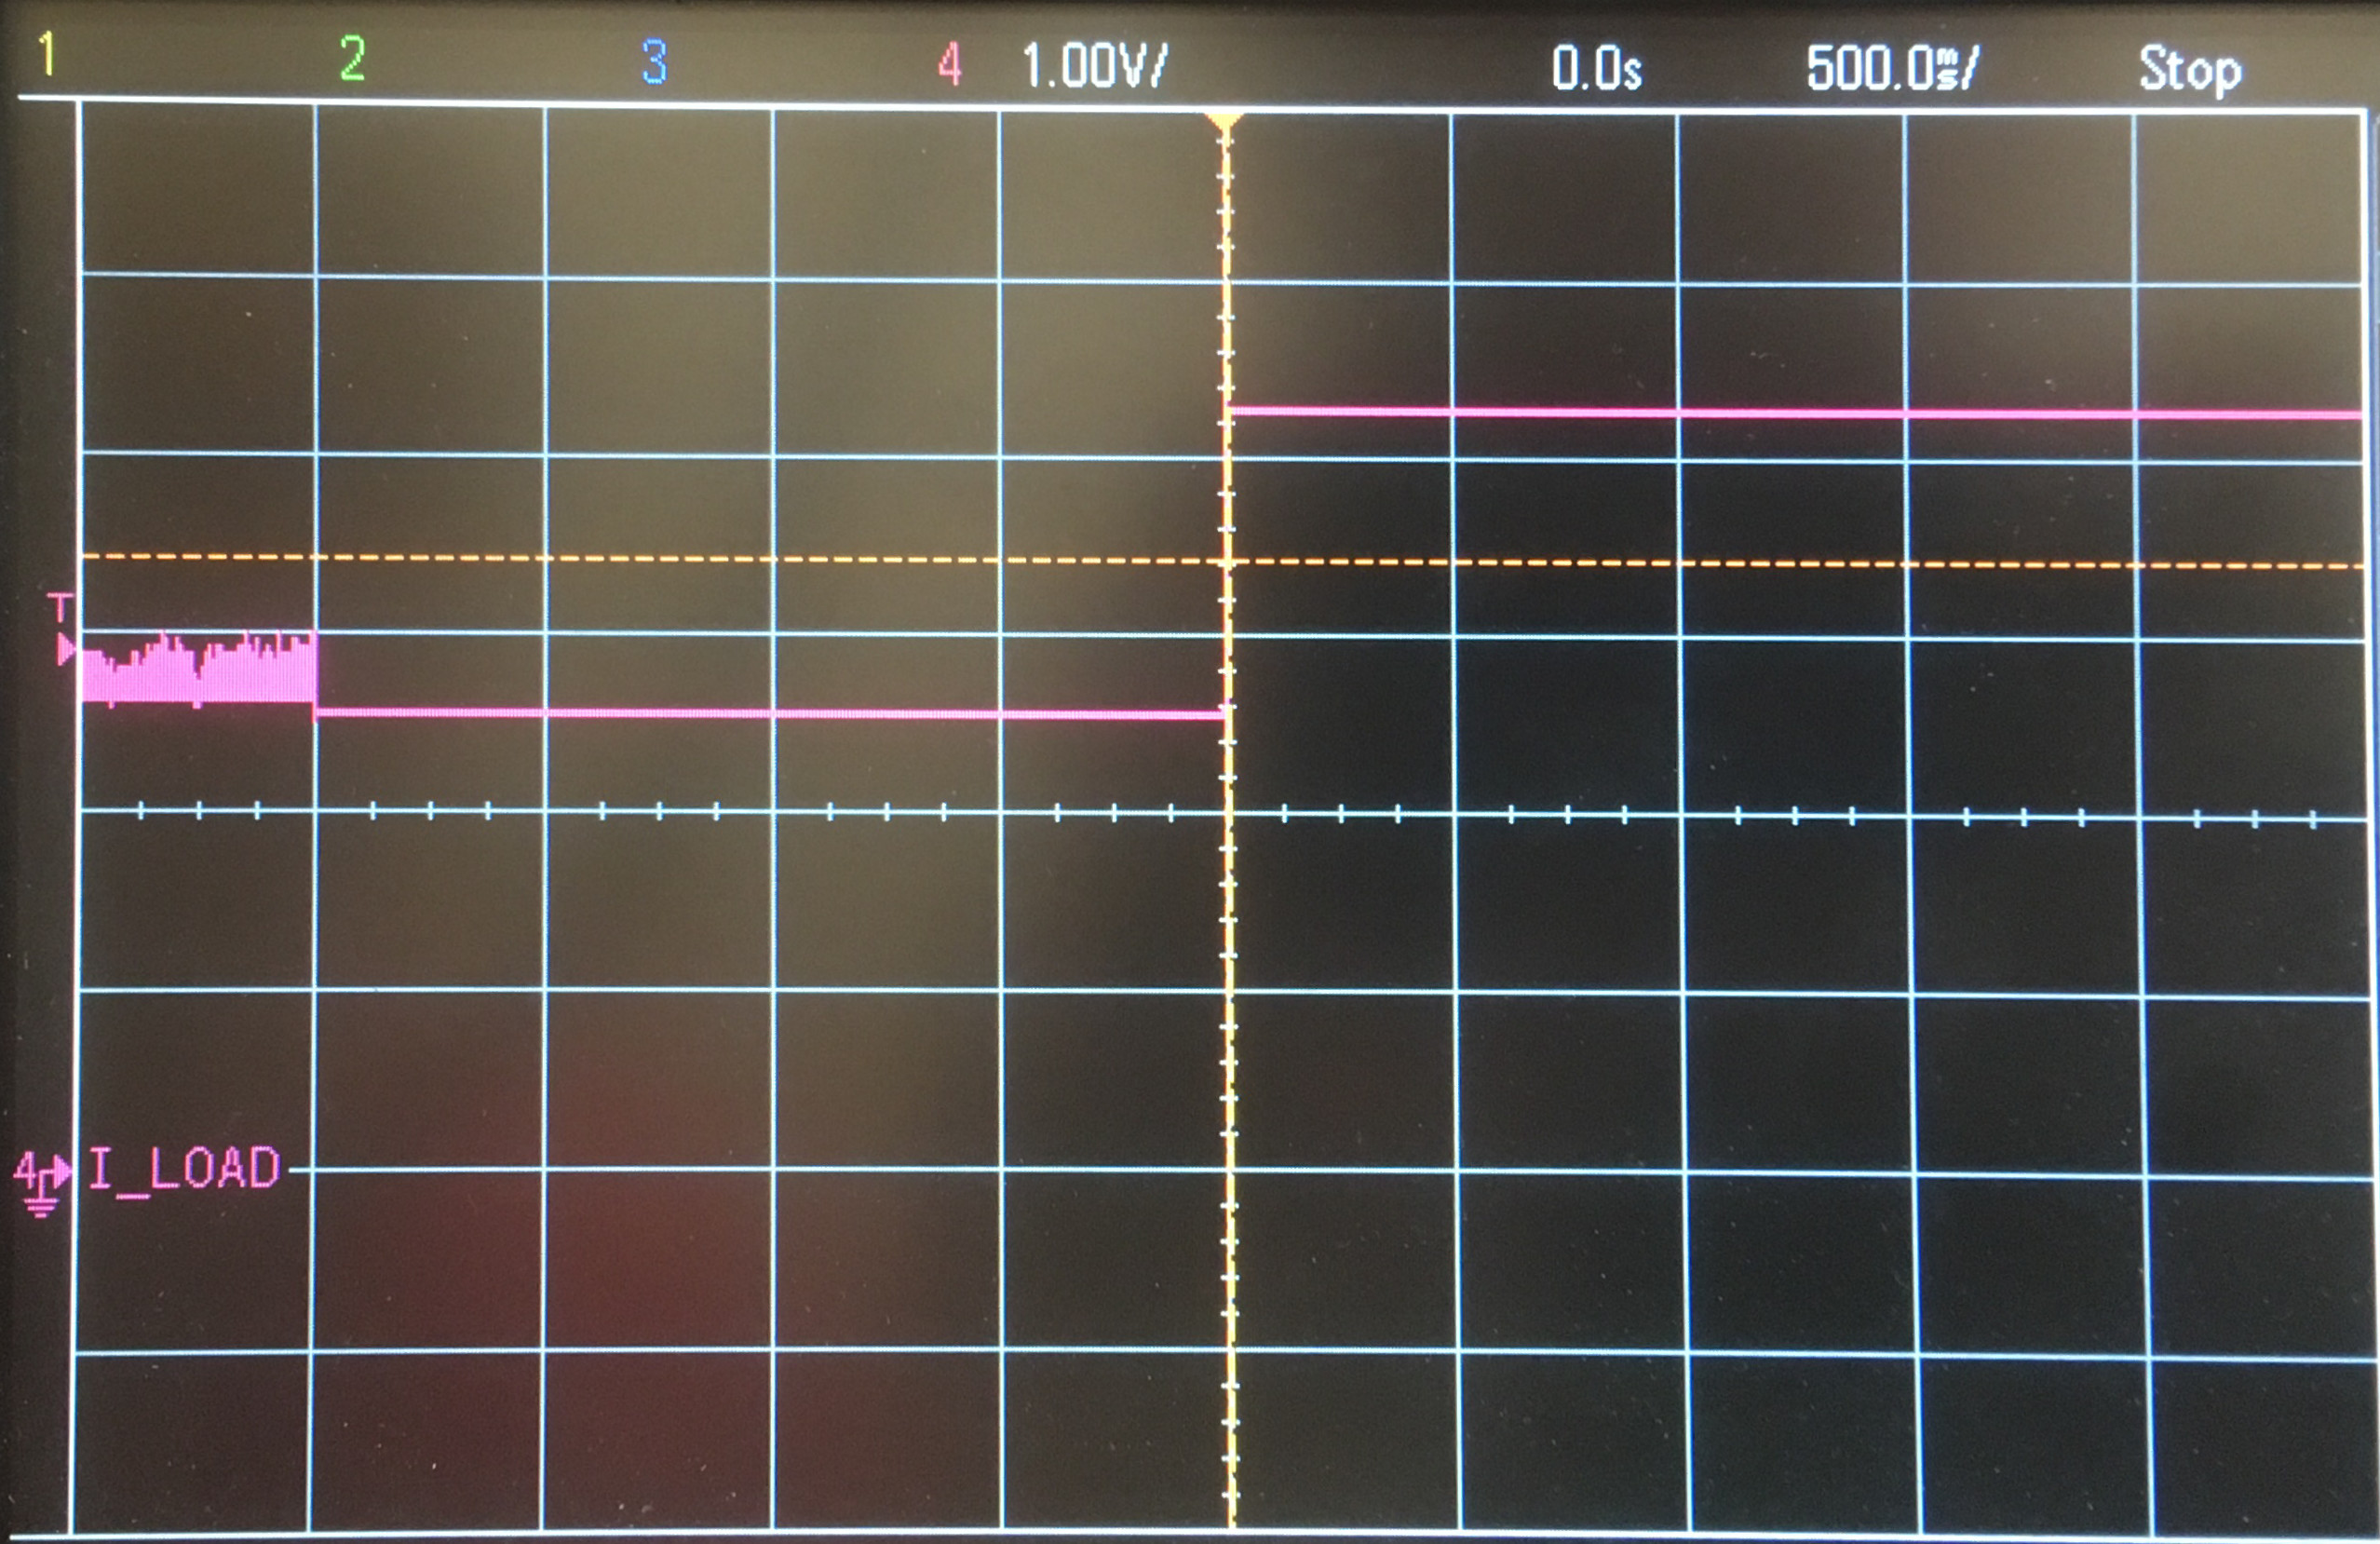
\includegraphics[width=0.8\linewidth]
        {./res/current_transient/regain_of_lock.jpg}
    \caption[Regain of lock transient current]{
        Currently 007 cannot regain lock, but 008 can.
        Note that during the loss of lock stage, 008 is much more noisy.
        Measured on 008.
    }
\end{figure}


\end{document}
